\chapter{基于手机GPU加速和离线模型压缩的能效优化}
\label{chapter:chapter3}
%表格模式设置左对齐:
%第一行用\multicolumn{1}{|c|}{文本内容}

本章详细分析了卷积神经网络前向推断过程中所使用的基本算子,并对每一个基本算子分别给出了基于手机GPU和CPU的实现方式。基于这些基本算子,本文实现了构成CNN推断时库所需的各种网络层。然后,利用实现的CNN推断时库和已训练好的CNN模型权重在手机平台上重构了LeNet-5和AlexNet,并分析比较了CPU版本和GPU版本两种实现方式的能效。最后,本章描述了基于“剪枝-重训”的权重压缩方法,并使用该方法对卷积神经网络中占存储量主要部分的全连接层权重进行了压缩。对于压缩后的CNN模型,本章进一步使用稀疏矩阵向量乘(SpMV)代替密集矩阵的内积运算。最后,与CNNdroid\cite{latifi2016cnndroid}的对比实验进一步分析了本文所开发CNN推断时库的性能。

\section{CNN前向推断基本算子的分解与实现}
\label{chapter:chapter3-1}
卷积神经网络的前向推断过程主要涉及卷积层、池化层、全连接层和激活层等的前向传播,故而对CNN前向推断基本算子的分解即需剖析实现这些层所需的基本算子。下面针对每层的基本算子,详细介绍其作用机理并分析比较基于手机GPU和CPU实现版本的能效。

\subsection{全连接层基本算子}

\begin{figure}[htbp]
    \begin{center}
    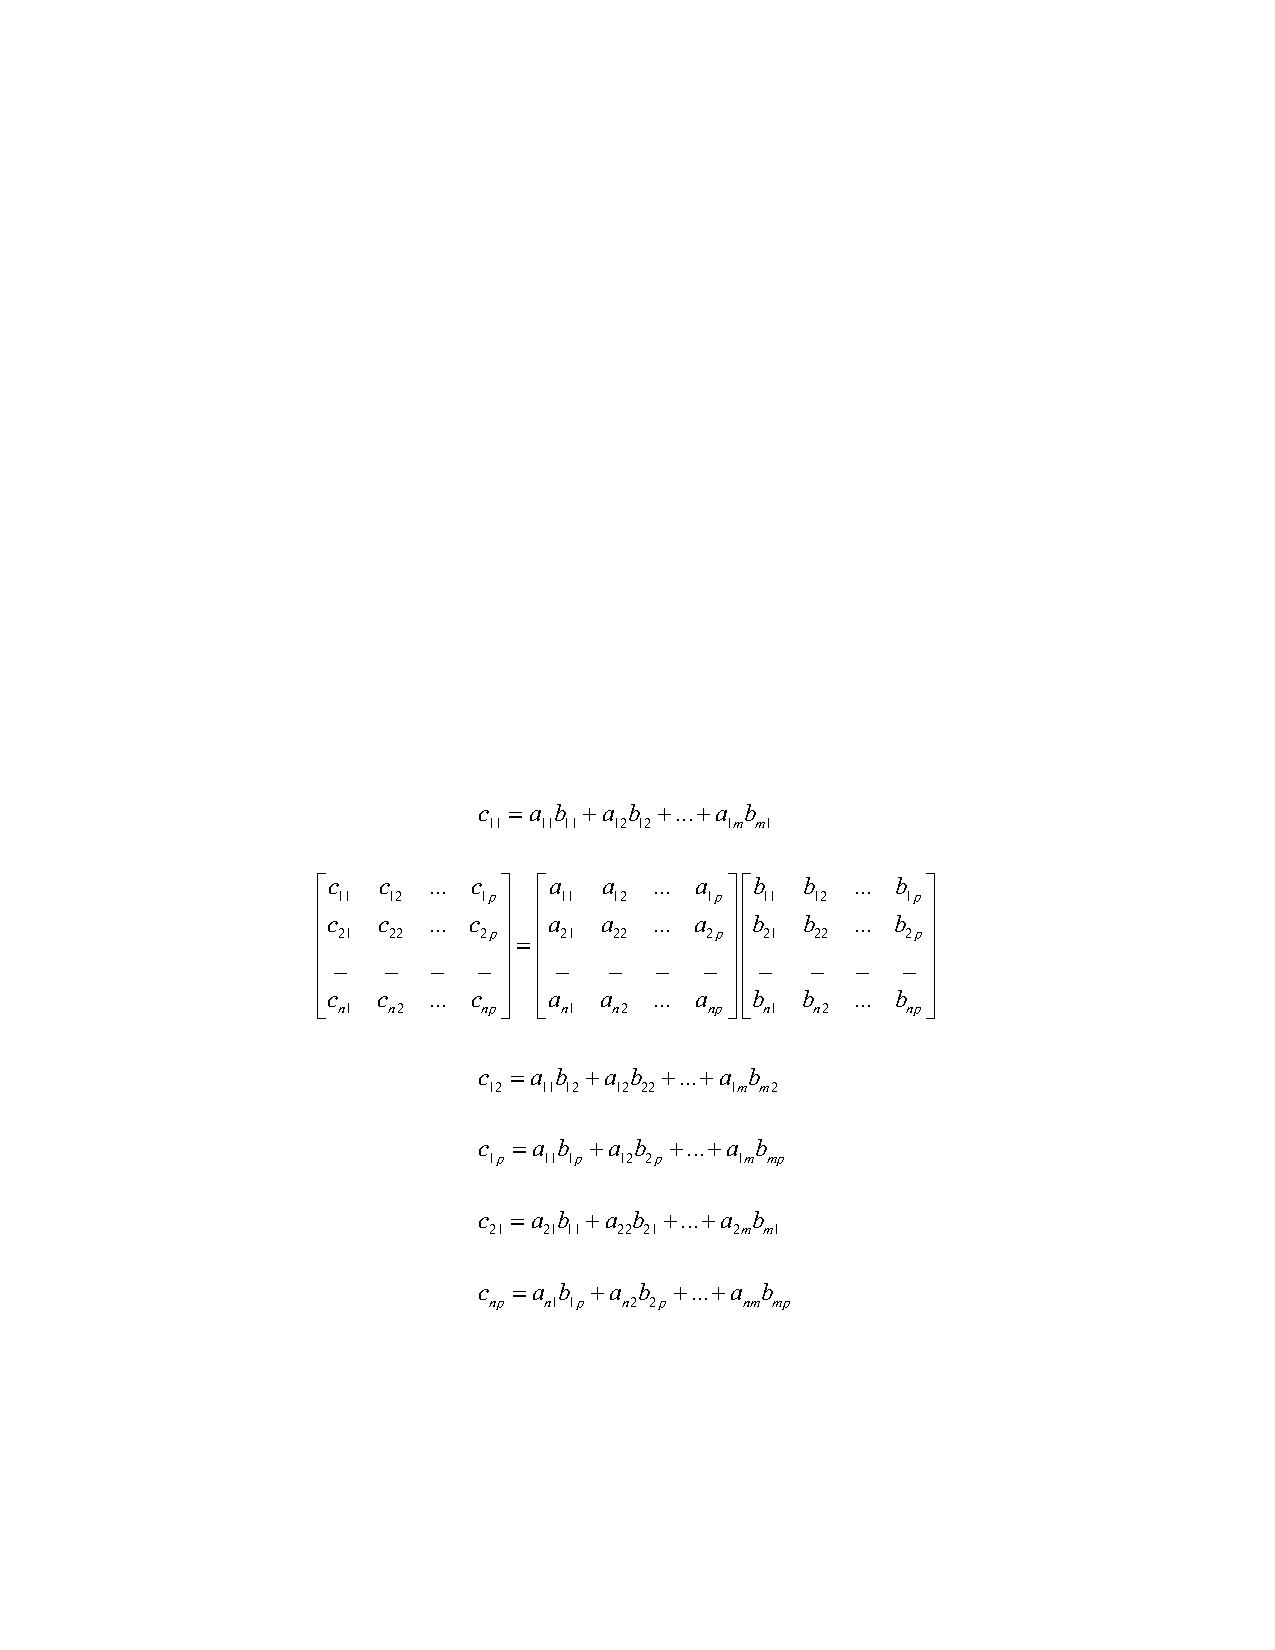
\includegraphics[height=0.5\textwidth]{figures/mat.pdf}
    \end{center}
    \caption{矩阵乘法定义}\label{figure:figure8}
\end{figure}

矩阵乘法操作是全连接层用到的主要基本算子,而且其在本文的卷积层实现中也被涉及,所以在此先介绍矩阵乘法于手机GPU和CPU上的实现。图\ref{figure:figure8}给出了矩阵乘法的定义。根据定义可得CPU版本的矩阵乘法实现伪代码如下:

\begin{algorithm}[htbp]
  \small
  \SetAlgoLined
  \KwData{mat\_left, row\_left, col\_left, mat\_right, row\_right, col\_right, bias, result}
    \begin{spacing}{0.9}
  \For{i in 0 ... row\_left-1}{
    \For{j in 0 ... col\_right-1}{
            res = 0\;
      \For{k in 0 ... col\_left-1}{
        res +=
        mat\_left[i * col\_left + k] *
        mat\_right[k * col\_right + j]\;
      }
    res += bias[i]\;
        result[i * col\_right + j] = res;
    }
  }
    \end{spacing}
  \caption{CPU版本矩阵乘法}
  \label{algo:algorithm1}
\end{algorithm}

基于OpenCL异构编程框架,下面给出GPU版本的矩阵乘法实现。将CPU版本中第一重和第二重循环的次数分别设置为核函数的全局工作空间大小,可将CPU版本代码直接改成GPU版本的标量形式,伪代码表示如下:

\begin{algorithm}[htbp]
  \small
  \SetAlgoLined
  \KwData{mat\_left, mat\_right, col\_left, bias, result}
    \begin{spacing}{0.9}
    初始化res的值为0\;
  i = get\_global\_id(0)\;
  j = get\_global\_id(1)\;
  col\_right = get\_global\_size(1)\;
  \For{k in 0 ... col\_left-1}{
    res += mat\_left[i * col\_left + k] * mat\_right[k * col\_right + j]\;
  }
    res += bias[i]\;
  result[i * col\_right + j] = res\;
    \end{spacing}
  \caption{GPU版本矩阵乘法(标量形式)}
  \label{algo:algorithm2}
\end{algorithm}

上述伪代码中\texttt{get\_global\_id(dim)}用于获得第\texttt{dim}维上的工作项全局ID,\texttt{get\_global\_size(dim)}用于获得第\texttt{dim}维上的全局工作项个数。GPU版本矩阵乘法的标量形式没有充分利用OpenCL的向量处理能力,这会造成一定的GPU并行计算性能损失。算法\ref{algo:algorithm3}给出了GPU版本矩阵乘法向量形式的核心伪代码实现。在向量形式实现版本中使用了\texttt{float4}向量数据类型,并通过OpenCL \texttt{dot()}函数完成对两个\texttt{float4}类型数据的一次内积操作。此处需要注意一点:因为对右矩阵不能使用\texttt{vload4()}函数连续读取数据,所以需要先读取所需的4个数据再将它们转换为一个\texttt{float4}向量类型,这样才能使得两个包含四元素的向量内积操作可以在一个时钟周期内完成。

\begin{algorithm}[htbp]
  \small
  \SetAlgoLined
  \KwData{mat\_left, mat\_right, col\_left, bias, result}
    \begin{spacing}{0.9}
    初始化res的值为0\;
    remain表示核函数剩余未处理的数据量\;
    \While{remain >= 4}{
        从mat\_left中使用vload函数取出四个数据组成float4向量类型tmp1\;
        从mat\_right中取出与tmp1对应的四个数据组成float4向量类型tmp2\;
        使用dot函数计算res的当前值:res += dot(tmp1, tmp2)\;
        设置mat\_left和mat\_right的下标偏移量\;
        更新剩余未处理的数据量:remain -= 4\;
    }
    \While{remain > 0} {
        从mat\_left中取出一个float数据tmp1\;
        从mat\_right中取出一个float数据tmp2\;
        更新res的当前值:res += tmp1 * tmp2\;
        设置mat\_left和mat\_right的下标偏移量\;
        更新剩余未处理的数据量:remain -= 1\;
    }
    将res加上对应偏置值并将结果赋值给result对应项\;
    \end{spacing}
  \caption{GPU版本矩阵乘法(向量形式)}
  \label{algo:algorithm3}
\end{algorithm}

基于ODROID-XU3实验平台,本文分析比较了上述三个矩阵乘法实现版本的能效。图\ref{figure:figure9}显示了$512\times1024$矩阵与$1024\times512$矩阵相乘的运行时间、能耗和平均功耗结果。

\begin{figure}[htbp]
    \begin{center}
    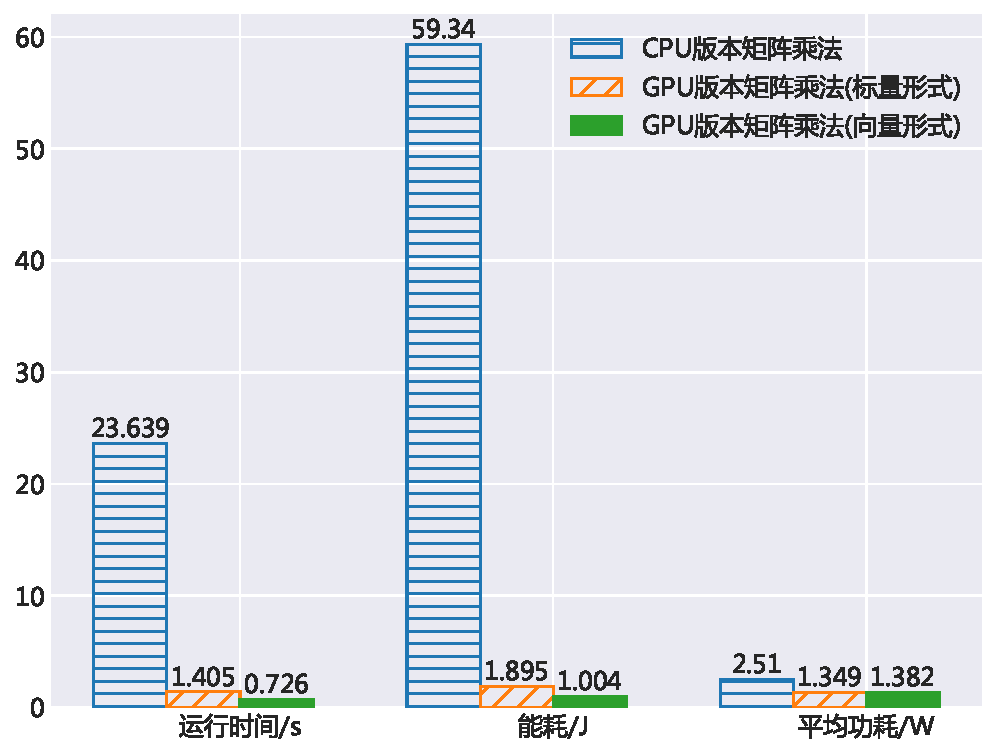
\includegraphics[height=0.4\textwidth]{figures/matmul.pdf}
    \end{center}
    \caption{矩阵乘法不同实现版本的运行时间、能耗和平均功耗对比}\label{figure:figure9}
\end{figure}

\begin{table}[htbp]
  \centering
  \caption{矩阵乘法不同实现版本的能效对比}
  \label{table:table1}
  \begin{tabular}{cc}
    \toprule
      实现版本 & EDP(Joules*seconds) \\
    \midrule
      CPU版本矩阵乘法 & 1402.763 \\
      GPU版本矩阵乘法(标量形式) & 2.663 \\
      GPU版本矩阵乘法(向量形式) & 0.729 \\
    \bottomrule
  \end{tabular}
\end{table}

由图\ref{figure:figure9}可知,使用手机GPU实现矩阵乘法可以明显提升运算性能并降低运行时能耗和功耗。对于$512\times1024$矩阵与$1024\times512$矩阵的乘积运算,相较于CPU实现版本,GPU的标量实现形式加速比为16.82。另一方面,通过比较GPU版本矩阵乘法的标量实现形式和向量实现形式,可以发现使用OpenCL的\texttt{float4}向量数据类型可以再获得约2倍的性能提升并可进一步降低运行时能耗。观察图\ref{figure:figure9}显示的平均功耗信息可知,使用手机CPU执行矩阵内积操作的功耗大约是使用手机GPU时的2倍。这也说明了在移动端SoC设计中,手机CPU功耗是高于GPU的。另外,与仅使用GPU标量数据类型相比,使用GPU向量数据类型执行SIMD(单指令多数据流)指令时功耗会略有上升。由表\ref{table:table1}可知,GPU版本矩阵乘法在能效方面远高于CPU版本矩阵乘法,尤其在使用OpenCL向量数据类型实现时GPU版本的能效提升了近两千倍(EDP的定义见\ref{chapter:edp}节,其值越小说明能效越高)。

\subsection{卷积层基本算子}

卷积层的基本算子即为卷积操作,这在第二章进行了相关介绍。然而,为了提高卷积操作的执行性能,本文采用了\texttt{img2col}结合通用矩阵乘的实现方式。

根据第二章介绍的卷积操作可知,每次滑动卷积窗口,都需要将卷积核的每一个权重值与窗口对应处的图像数据值相乘,并将所有的乘积相加求和,整个操作过程非常类似于向量的内积运算。因此,理论上可以使用矩阵乘法实现卷积操作,这便是通过\texttt{img2col}操作实现的。

\begin{figure}[htb]
    \begin{center}
    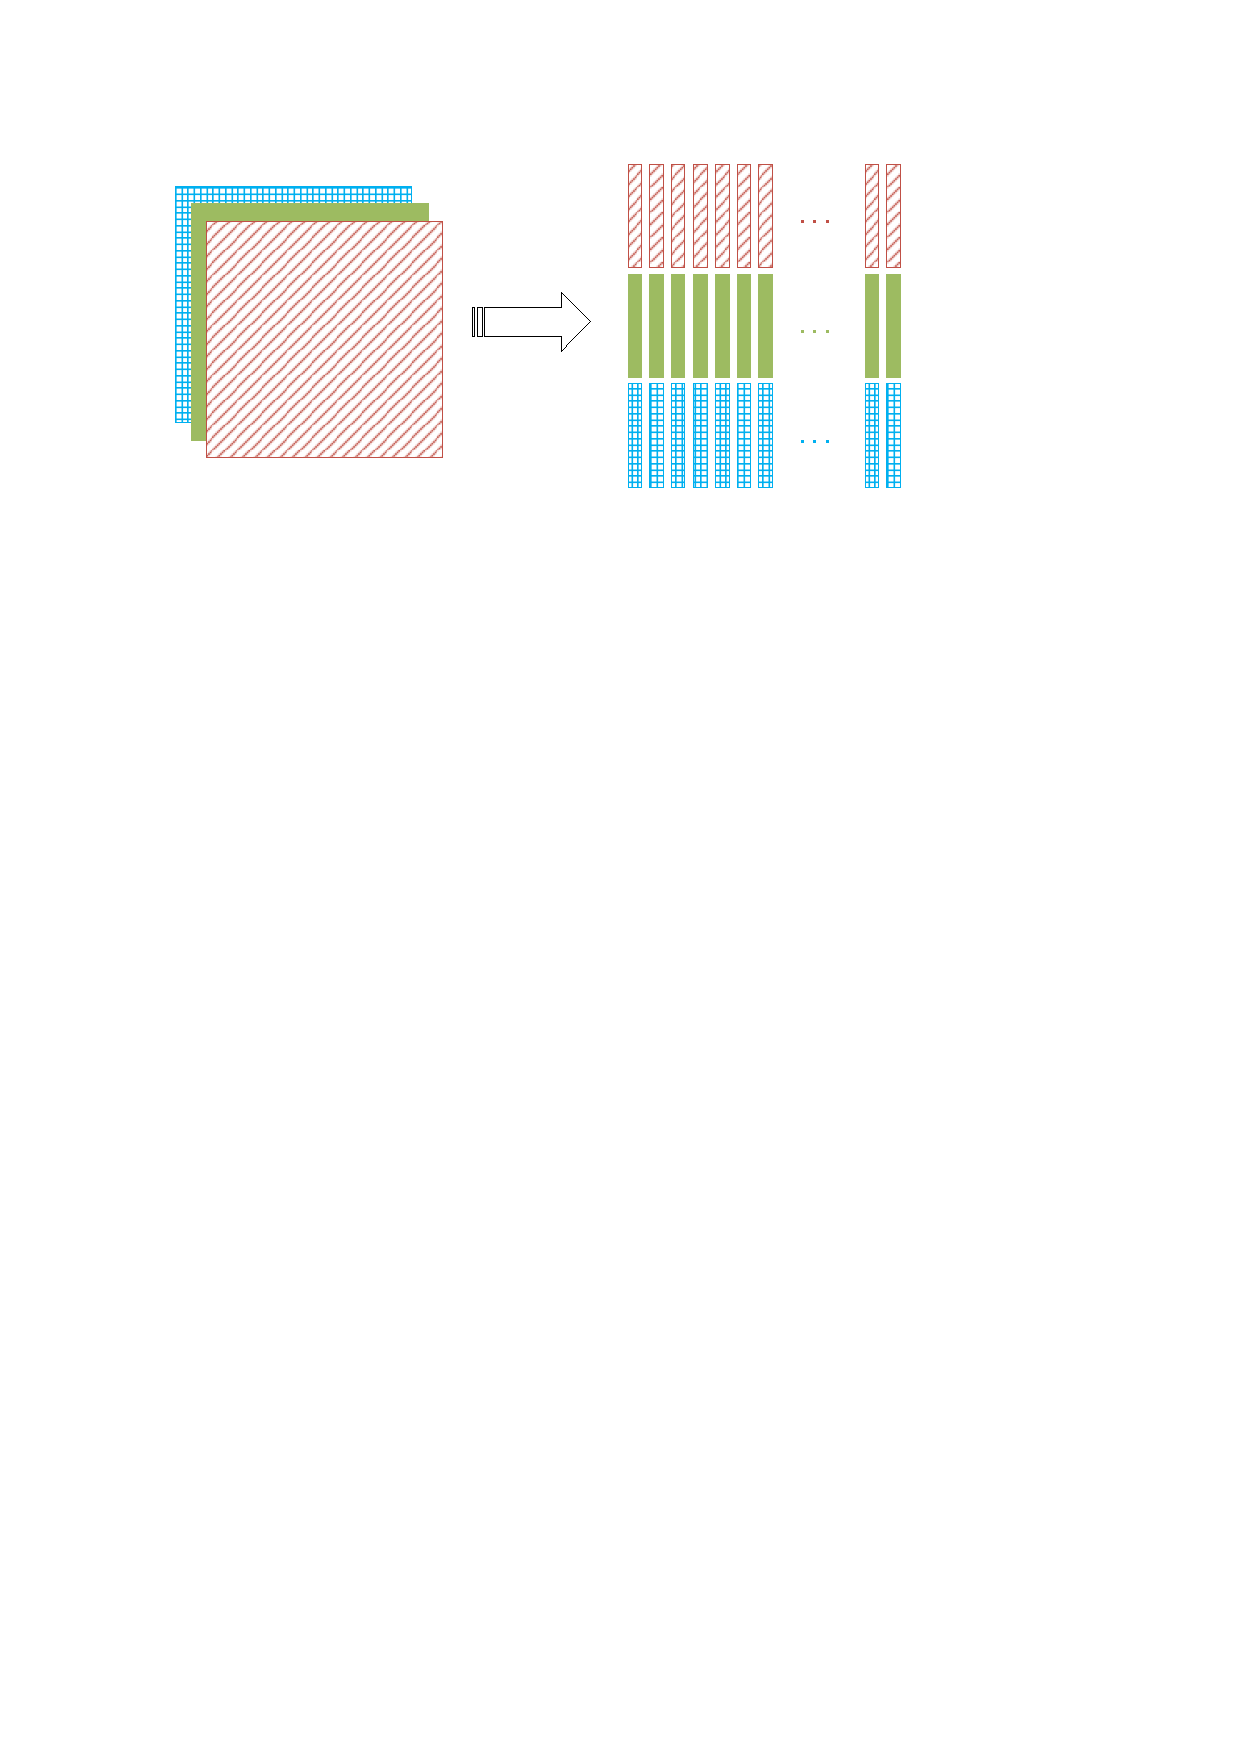
\includegraphics[height=0.3\textwidth]{figures/im2col.pdf}
    \end{center}
    \caption{\texttt{img2col}转换三通道输入特征图示例}\label{figure:figure10}
\end{figure}

将卷积操作转换为矩阵内积运算需要进行如下两步操作:(1)使用\texttt{img2col}将输入特征图转换为使用矩阵乘法实现卷积操作时所需的矩阵形式,图\ref{figure:figure10}给出了一个使用\texttt{img2col}将三通道输入特征图转换为所需输出矩阵的示例;(2)使用矩阵乘法将权重矩阵与第一步转化而来的矩阵进行相乘得到卷积输出结果。算法\ref{algo:algorithm4}详细描述了\texttt{img2col}的执行过程。

\begin{algorithm}[htbp]
  \small
  \SetAlgoLined
    \begin{spacing}{0.8}
    \KwData{channels, channel\_size, kernel\_h,kernel\_w, output\_h,output\_w}
    channels,channel\_size分别表示输入通道数和一个通道的数据量\;
    kernel\_h,kernel\_w分别表示卷积核的高度和宽度\;
  output\_h,output\_w分别表示卷积层输出特征图的高度和宽度\;
    \For{channel in 0 ... channels-1} {
        \For{kernel\_row in 0 ... kernel\_h-1} {
            \For{kernel\_col in 0 ... kernel\_w-1} {
                计算卷积核中第kernel\_row行首个操作区域在输入特征图上的行索引\;
                \For{output\_rows in output\_h ... 1} {
                    \If{计算得到的输入特征图的行值索引小于零或者大于输入特征图的高} {
                        \For{output\_cols in output\_w ... 1} {
                            将该行在输出矩阵上的位置置为0\;
                        }
                    } \Else {
                        计算卷积核中第kernel\_col列首个操作区域在输入特征图上的列索引\;
                        \For{output\_cols in output\_w ... 1} {
                            \If{输入特征图的列值索引大于等于零或者小于输入特征图的宽} {
                                将输入特征图上对应的区域放到输出矩阵上;
                            } \Else {
                                将该行该列在输出矩阵上的位置置为0\;
                            }
                            将输出列坐标移动到下一个卷积窗口\;
                        }
                    }
                    将输出行坐标移动到下一个卷积窗口\;
                }
            }
        }
        将输出矩阵偏移channel\_size以操作下一个输入通道的图像数据\;
    }
    \end{spacing}
  \caption{\texttt{img2col}核心操作伪代码}
  \label{algo:algorithm4}
\end{algorithm}

根据算法\ref{algo:algorithm4}描述的伪代码,本文分别于手机GPU和CPU上实现了\texttt{img2col}操作。为了比较\texttt{img2col}在手机GPU和CPU上的执行性能,本文基于ODROID-XU3平台测量了\texttt{img2col}在处理高度和宽度均为256、通道数为100的输入特征图(步长为1,卷积核大小为$3 \times 3$并且无padding处理)的运行时间、能耗和平均功耗,结果如图\ref{figure:figure11}所示。

\begin{figure}[htbp]
    \begin{center}
    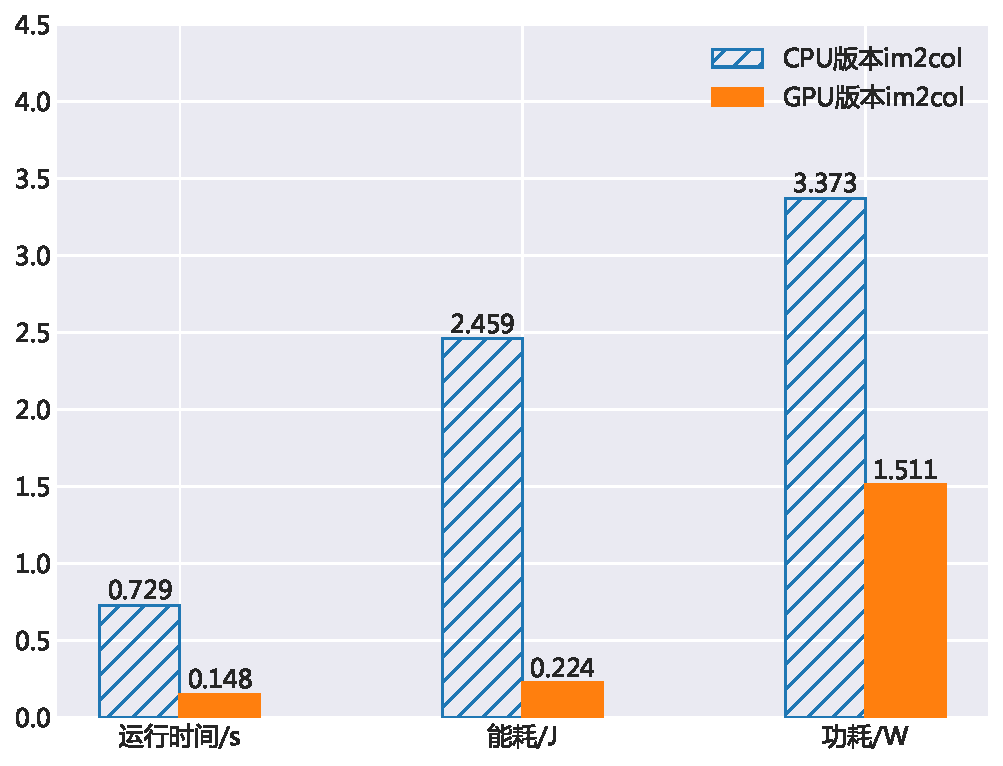
\includegraphics[height=0.4\textwidth]{figures/im2col_energy.pdf}
    \end{center}
    \caption{\texttt{img2col}不同实现版本的运行时间、能耗和平均功耗对比}\label{figure:figure11}
\end{figure}

由图\ref{figure:figure11}可知,在操作高度和宽度均为256、通道数为100的输入特征图时,相较于CPU版本的\texttt{img2col},GPU版本的\texttt{img2col}可使得执行速度提升5倍左右。与此同时,使用GPU执行\texttt{img2col}操作的能耗仅为使用CPU能耗的1/10,而平均功耗不到使用CPU时的1/2。表\ref{table:table2}显示了GPU版本\texttt{img2col}和CPU版本\texttt{img2col}的EDP值。对比两者的EDP值可知,基于GPU实现的\texttt{img2col}可以将能效提升54倍以上。

\begin{table}[htbp]
  \centering
  \caption{\texttt{img2col}不同实现版本的能效对比}
  \label{table:table2}
  \begin{tabular}{cc}
    \toprule
      实现版本 & EDP(Joules*seconds) \\
    \midrule
      CPU版本im2col & 1.792 \\
      GPU版本im2col & 0.033 \\
    \bottomrule
  \end{tabular}
\end{table}


\subsection{池化层基本算子}

显然,池化层的基本算子即为池化单元。由\ref{chapter:chapter2-1-2}节可知,最大池化是目前研究工作中最为常用的池化单元,因此本文主要实现了最大池化操作。根据第\ref{chapter:chapter2-1-2}节中对最大池化操作的自然语言描述,可形成如算法\ref{algo:algorithm5}所示的最大池化操作伪代码。同样地,本文于手机GPU和CPU上分别实现了算法\ref{algo:algorithm5}所描述的伪代码。

\begin{algorithm}[htbp]
  \small
  \SetAlgoLined
    \begin{spacing}{0.8}
    \KwData{channels, pooled\_h, pooled\_w}
    channels表示输入通道数\;
    pooled\_h和pooled\_w分别表示池化输出矩阵的高度和宽度\;
    \For{c in 0 ... channels-1} {
        \For{ph in 0 ... pooled\_h-1} {
            \For{pw in 0 ... pooled\_w-1} {
                计算本次池化窗口的行操作起始位置hstart和终止位置hend\;
                计算本次池化窗口的列操作起始位置wstart和终止位置wend\;
                确保本次行列操作起始位置hstart和wstart均为非负值\;
                计算本次池化操作输出矩阵的对应下标pool\_index\;
                将本次池化窗口左上角第一个值赋给输出矩阵下标为pool\_index的项\;

                \For{h in hstart ... hend-1} {
                    \For{w in wstart ... wend-1} {
                      利用上面两重循环,遍历本次池化窗口中每一个值value\;
                        将value与输出矩阵下标为pool\_index的项做比较\;
                      将两者较大值重新赋值给输出矩阵下标为pool\_index的项\;
                    }
                }
            }
        }
        将输入特征图和输出矩阵均偏移到下一个通道\;
    }
    \end{spacing}
  \caption{最大池化核心操作伪代码}
  \label{algo:algorithm5}
\end{algorithm}

%\begin{figure}[htbp]
%\begin{minipage}[b]{.6\linewidth}
%    \begin{center}
%    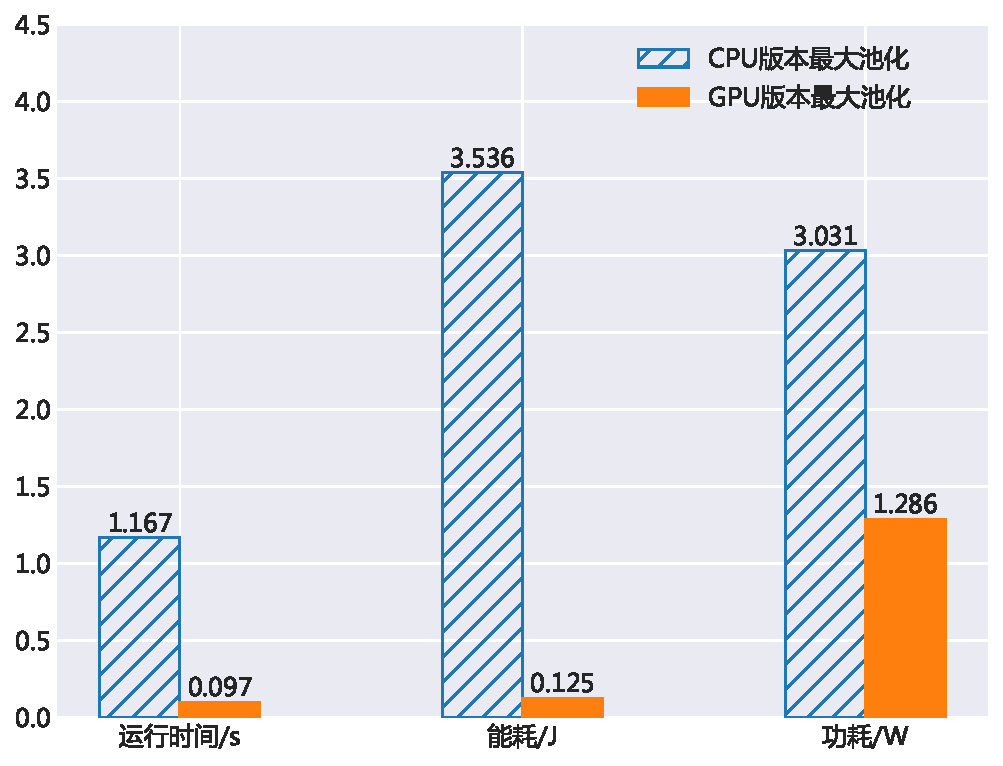
\includegraphics[height=0.65\textwidth]{figures/pool_energy.pdf}
%    \end{center}
%    \captionsetup{font={small}}
%    \caption{最大池化不同实现版本的运行时间、\\能耗和平均功耗对比}\label{figure:figure12}
%\end{minipage}
%\begin{minipage}[b]{.4\linewidth}
%\centering
%\resizebox{1.0\textwidth}{!}{
%\begin{tabular}{cc}
%    \toprule
%      实现版本 & EDP(Joules*seconds) \\
%    \midrule
%      CPU版本最大池化 & 4.125 \\
%      GPU版本最大池化 & 0.012 \\
%    \bottomrule
%\end{tabular}
%}
%\captionsetup{font={small}}
%\captionof{table}{最大池化不同实现版本的\\能效对比}\label{table:table3}
%\end{minipage}
%\end{figure}

对于一张高度和宽度均为256、通道数为100的输入特征图,本文测量了其在ODROID-XU3平台上进行最大池化操作所需的运行时间、能耗和平均功耗。实验中,池化操作的步长取为1、池化核大小取为$3 \times 3$,并且不进行padding处理,测量结果如图\ref{figure:figure12}所示。

由图\ref{figure:figure12}可知,使用GPU进行最大池化操作不仅可以将运算速度提升12倍还可以把能耗降为使用CPU时的1/28。最大池化在CPU和GPU上执行的功耗特征与\texttt{img2col}类似,即GPU版本最大池化平均功耗不足CPU版本的一半。表\ref{table:table3}从能效的角度分析了最大池化在不同计算设备上的表现,即GPU版本最大池化的能效要高出CPU版本约340余倍。

\begin{figure}[htb]
    \begin{center}
    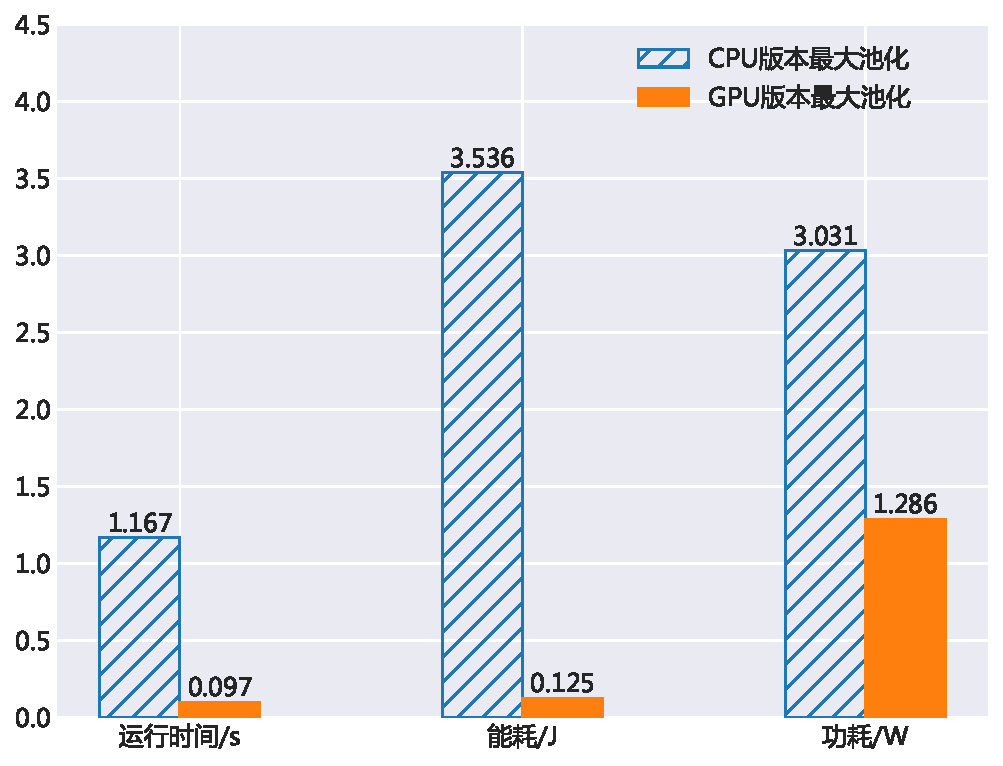
\includegraphics[height=0.4\textwidth]{figures/pool_energy.pdf}
    \end{center}
    \caption{最大池化不同实现版本的运行时间、能耗和平均功耗对比}\label{figure:figure12}
\end{figure}

\begin{table}[htbp]
  \centering
  \caption{最大池化不同实现版本的能效对比}
  \label{table:table3}
  \begin{tabular}{cc}
    \toprule
      实现版本 & EDP(Joules*seconds) \\
    \midrule
      CPU版本最大池化 & 4.125 \\
      GPU版本最大池化 & 0.012 \\
    \bottomrule
  \end{tabular}
\end{table}


\subsection{激活层基本算子}

正如\ref{chapter:chapter2-1-4}节所述,激活层主要使用非线性激活函数对输入数据进行处理,故而激活层的基本算子即为所使用的激活函数。在具体实现中,可选的激活函数主要有Relu函数、Sigmod函数以及双曲正切函数等。选定激活函数\texttt{activation\_fun()},激活层基本算子的实现伪代码可表示如下:

\begin{algorithm}[htbp]
  \small
  \SetAlgoLined
  \KwData{data, length}
  \For{i in 0 ... length-1}{
        data[i]=activation\_fun(data[i])\;
  }
  \caption{激活层基本算子实现伪代码}
  \label{algo:algorithm6}
\end{algorithm}

根据算法\ref{algo:algorithm6}所描述的实现逻辑,本文分别实现了基于手机GPU和CPU的激活操作。图\ref{figure:figure13}显示了Relu激活算子分别于手机GPU和CPU上处理$100 \times 256 \times 256 $个输入数据时的运行时间、能耗和平均功耗。

\begin{figure}[htb]
    \begin{center}
    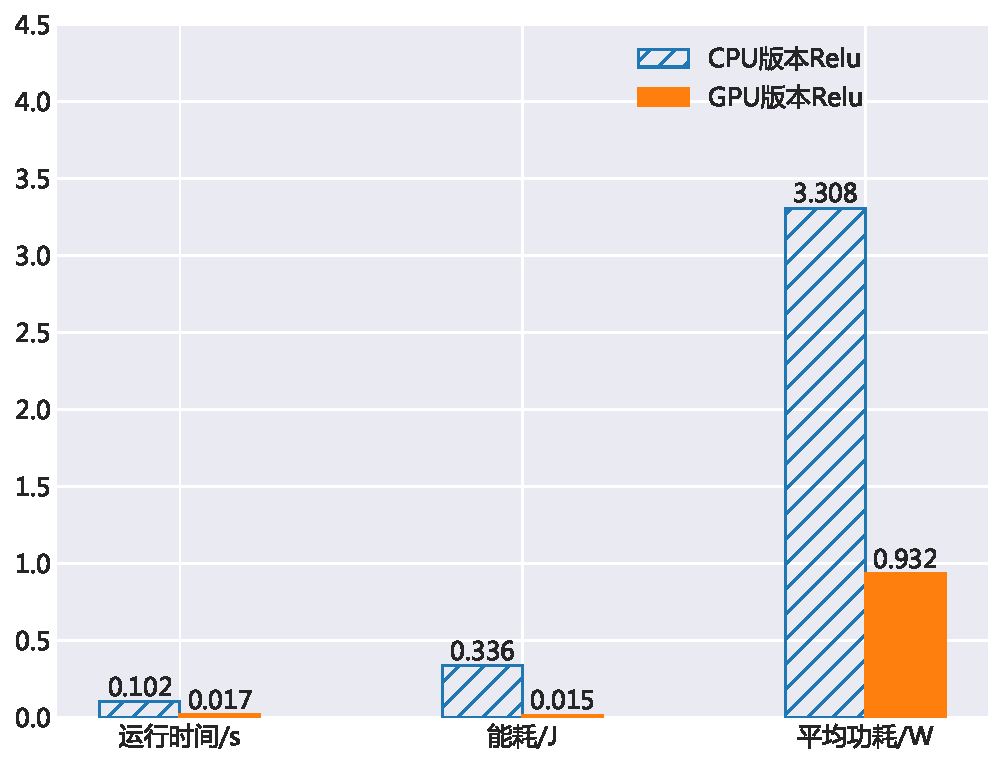
\includegraphics[height=0.4\textwidth]{figures/relu_energy.pdf}
    \end{center}
    \caption{Relu激活算子不同实现版本的运行时间、能耗和平均功耗对比}\label{figure:figure13}
\end{figure}

从图\ref{figure:figure13}可以看出,在输入数据量为$100 \times 256 \times 256 $时,GPU版本Relu激活算子的执行速度可比CPU版本的快6倍,并同时可降低22倍的能耗和3.5倍的功耗。表\ref{table:table4}给出Relu激活算子分别在CPU和GPU上运行时的能效。其中,CPU版本Relu激活算子的EDP为0.034,而GPU版本Relu激活算子的EDP仅为0.0003。根据EDP值越小能效越高的度量标准可知,在输入数据量为$100 \times 256 \times 256 $时,Relu激活算子在GPU上的运行时能效是其在CPU上的100多倍。

\begin{table}[htbp]
  \centering
  \caption{Relu激活算子不同实现版本的能效对比}
  \label{table:table4}
  \begin{tabular}{cc}
    \toprule
      实现版本 & EDP(Joules*seconds) \\
    \midrule
      CPU版本Relu激活算子 & 0.034 \\
      GPU版本Relu激活算子 & 0.0003 \\
    \bottomrule
  \end{tabular}
\end{table}

%\begin{figure}[htbp]
%\begin{minipage}[b]{.6\linewidth}
%    \begin{center}
%    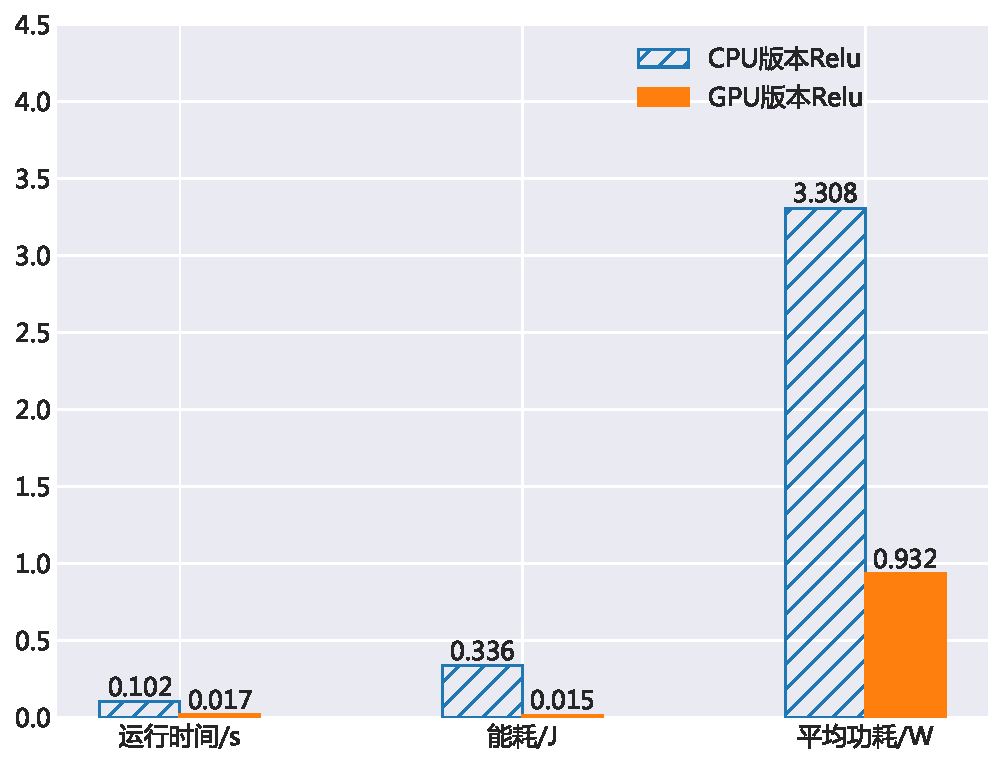
\includegraphics[height=0.65\textwidth]{figures/relu_energy.pdf}
%    \end{center}
%    \captionsetup{font={small}}
%    \caption{Relu激活算子不同实现版本的运行时间、\\ 能耗和平均功耗对比}\label{figure:figure13}
%\end{minipage}
%\begin{minipage}[b]{.4\linewidth}
%\centering
%\resizebox{1.0\textwidth}{!}{
%\begin{tabular}{cc}
%    \toprule
%      实现版本 & EDP(Joules*seconds) \\
%    \midrule
%      CPU版本Relu激活算子 & 0.034 \\
%      GPU版本Relu激活算子 & 0.0003 \\
%    \bottomrule
%\end{tabular}
%}
%\captionsetup{font={small}}
%\captionof{table}{Relu激活算子不同实现版本的能效对比}\label{table:table4}
%\end{minipage}
%\end{figure}

\section{基于手机GPU加速的CNN前向推断}

基于\ref{chapter:chapter3-1}节对CNN前向推断过程中所涉及基本算子的分解与实现,本文设计了一套可使用手机GPU或CPU执行CNN前向推断的运行时库。该CNN推断时库主要包括了卷积层、池化层、全连接层和激活层等网络层的实现。利用所设计的CNN推断时库,本章节于手机端重构了LeNet-5模型和AlexNet模型,并分析比较了两个模型在手机GPU和CPU上运行时的能效特征。

\subsection{预训练CNN模型权重参数解析}
\label{chapter:chapter321}

\begin{figure}[htbp]
    \begin{center}
    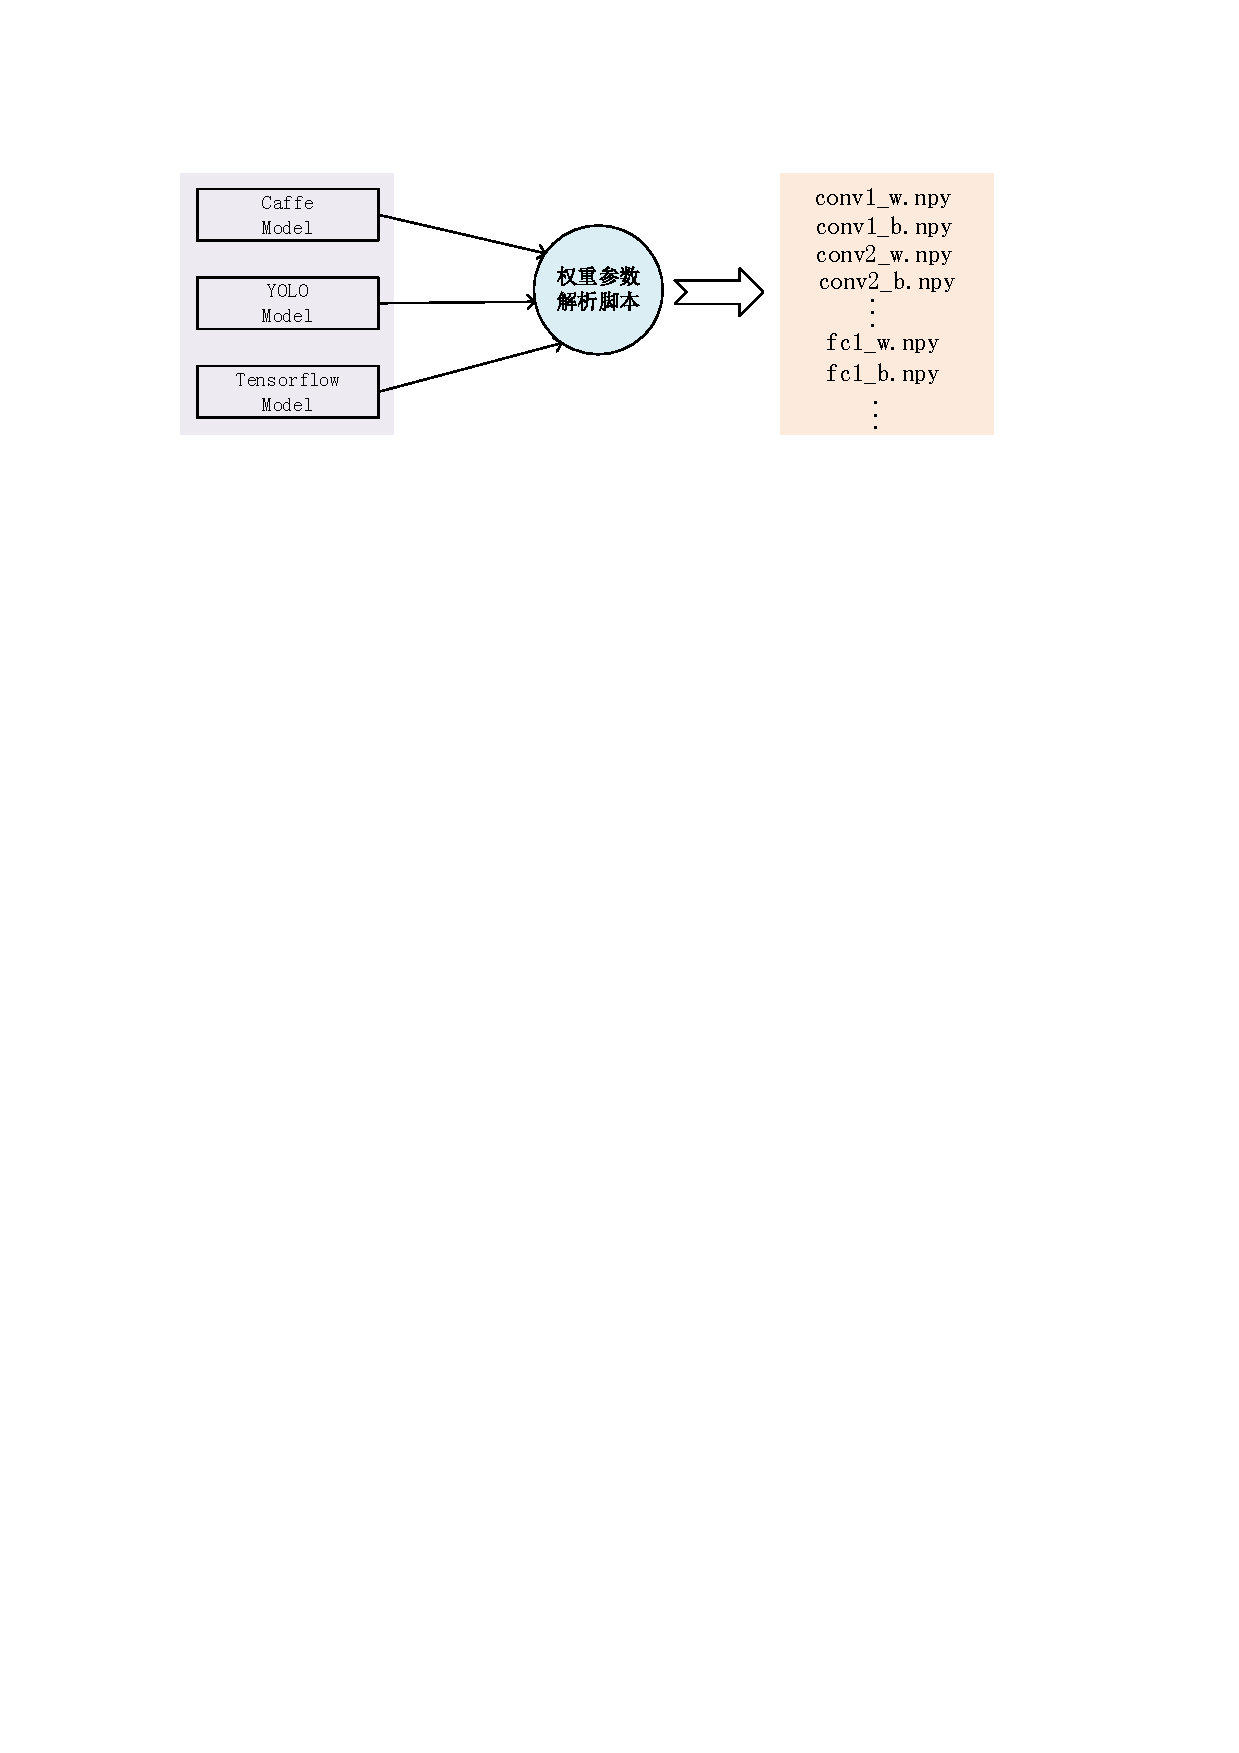
\includegraphics{figures/weight.pdf}
    \end{center}
    \caption{CNN模型权重参数解析流程}\label{figure:figure14}
\end{figure}

解析预训练CNN模型权重参数是在手机端重构卷积神经网络前向推断过程的首要条件,本文针对Caffe、YOLO和Tensorflow等深度学习框架所训练的CNN模型给出了权重解析的python脚本。该脚本可以提取预训练CNN模型的每层权重参数(权值矩阵和偏置矩阵等),并将这些权重参数分层保存为二进制文件格式,整个流程如图\ref{figure:figure14}所示。

\subsection{LeNet-5模型于手机端的重构}

\begin{figure}[htbp]
    \centering
    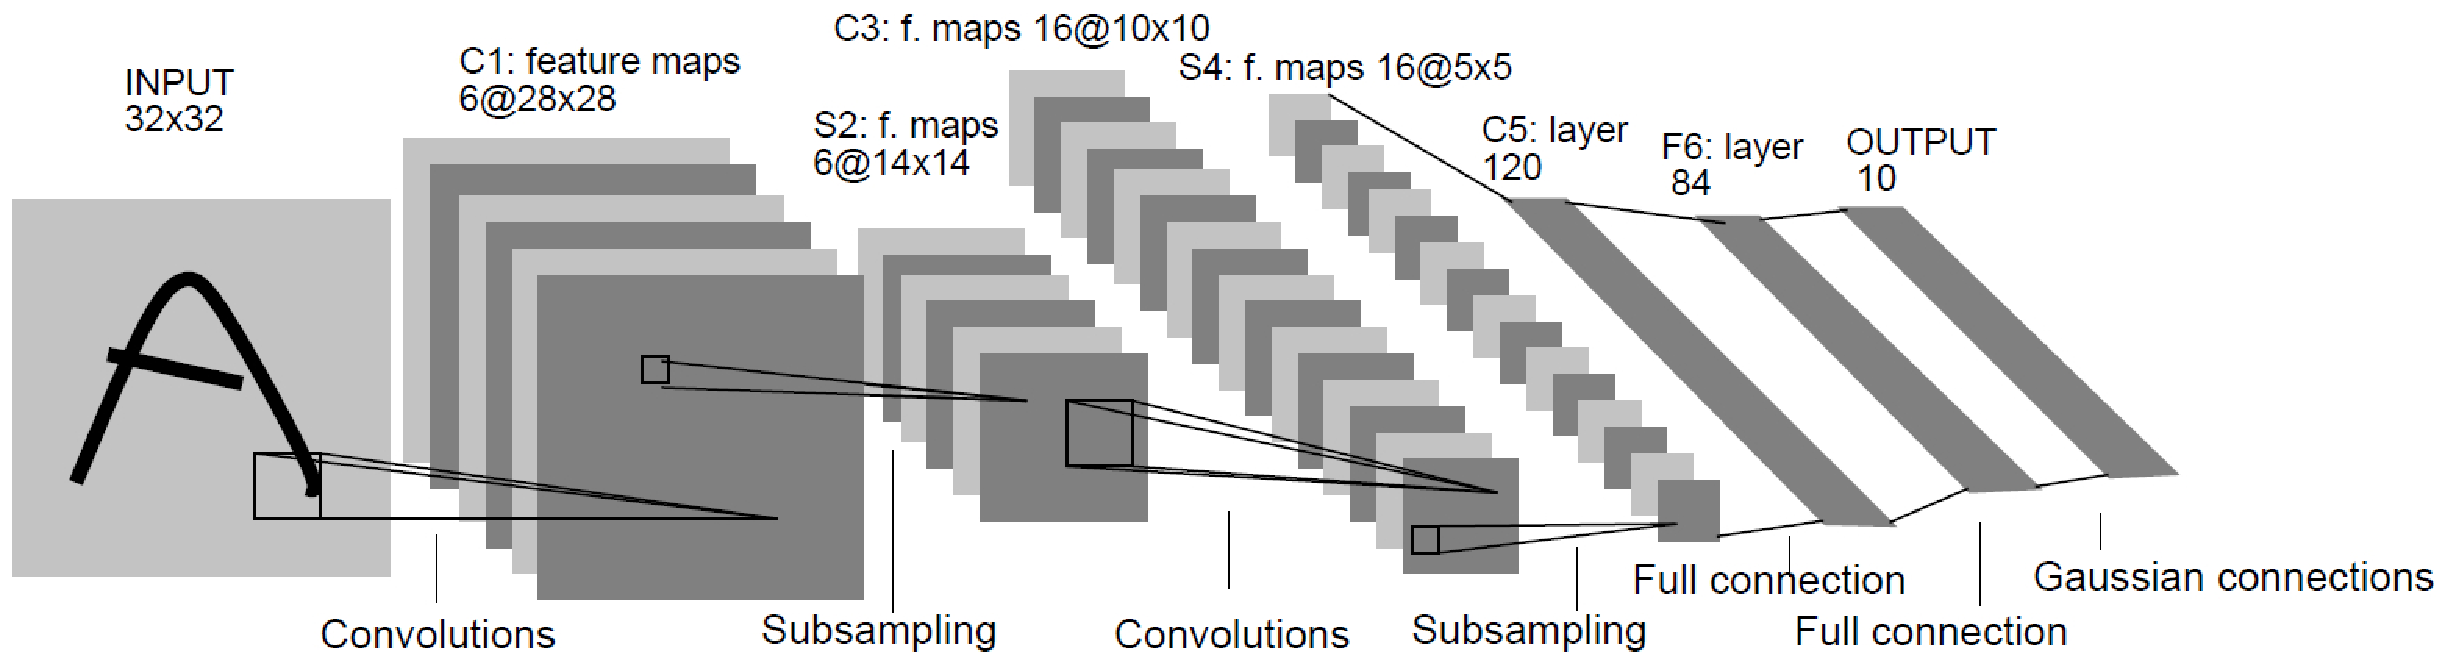
\includegraphics[width=1.0\textwidth]{figures/lenet.pdf}
    \caption{LeNet-5模型结构示意图 \cite{lecun1998gradient}}\label{figure:figure15}
\end{figure}

LeNet-5是由卷积神经网络之父Yan LeCun提出的,其主要用于手写字符的识别与分类。原始的LeNet-5模型主要由2个卷积层、2个池化层、1个全连接层以及1个高斯连接层组成,如图\ref{figure:figure15}所示。本文所采用的LeNet-5模型将最后一层高斯连接层替换为了全连接层,且在MNIST数据集\cite{lecun.com}上的预测精度可达99.1\%。表\ref{table:table5}描述了本文所采用的LeNet-5模型结构中卷积层和全连接层的参数信息。

\vspace{-1.5em}
\begin{table}[htbp]
  \centering
  \caption{LeNet-5模型结构中的卷积层和全连接层}
  \label{table:table5}
\resizebox{1.0\textwidth}{!}{
  \begin{tabular}{ccc}
    \toprule
      名称 & 类型 & 描述\\
    \midrule
      conv1 & 卷积层 & 输入:$1\times28\times28$,卷积核:$20\times1\times5\times5$,步长:1,padding:0,输出:$20\times24\times24$ \\
      conv2 & 卷积层 & 输入:$20\times12\times12$,卷积核:$50\times20\times5\times5$,步长:1,padding:0,输出:$50\times8\times8$\\
      ip1 & 全连接层 & 输入:800, 输出:500 \\
      ip2 & 全连接层 & 输入:500, 输出:10 \\
    \bottomrule
  \end{tabular}
}
\end{table}
\vspace{-0.5em}

利用\ref{chapter:chapter321}节的权重解析脚本,可获取到LeNet-5模型各层的权重矩阵。基于这些权重矩阵,本文分别于手机GPU和CPU上重构了LeNet-5模型,图\ref{figure:figure16}显示了LeNet-5模型在ODROID-XU3平台上进行单张图片前向推断所需的运行时间、能耗和平均功耗。

\begin{figure}[htbp]
    \centering
    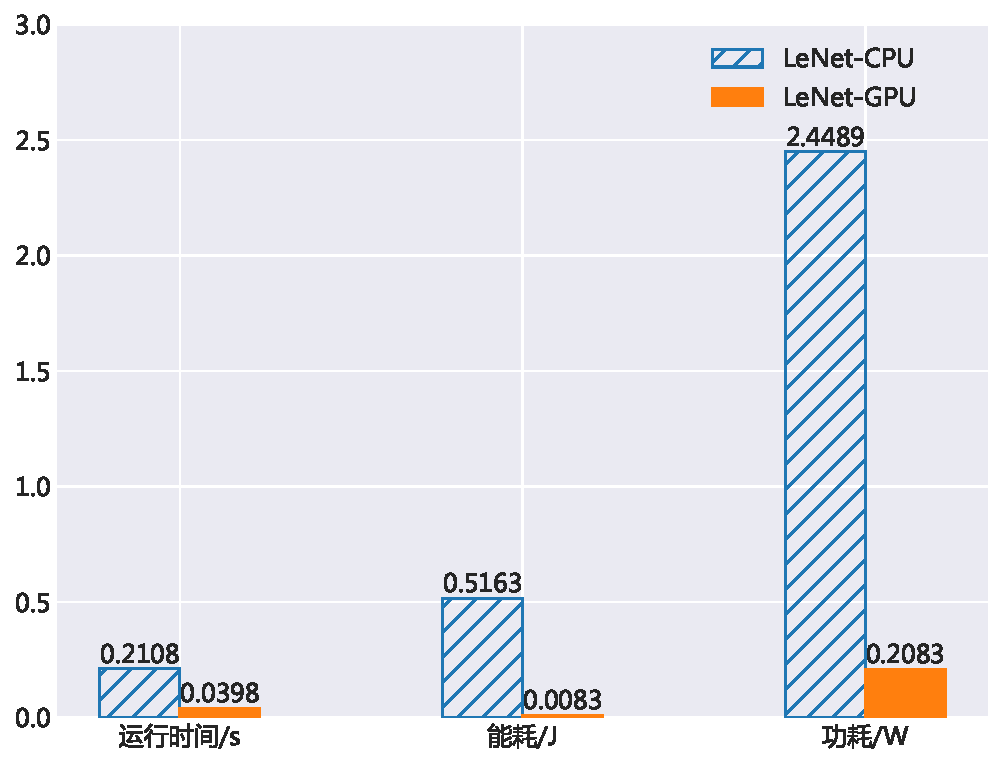
\includegraphics[height=0.4\textwidth]{figures/lenet_energy.pdf}
    \caption{LeNet-5单张图片推断运行时间、能耗和平均功耗对比}\label{figure:figure16}
\end{figure}

由图\ref{figure:figure16}可知,LeNet-5模型在手机GPU上进行前向推断的执行速度是在手机CPU上的11倍以上,并且可以节省120多倍的能耗。根据表\ref{table:table6}显示的LeNet-5模型分别于手机GPU和CPU上运行时EDP值可知,使用手机GPU进行LeNet-5的前向推断可以将能效提升1400倍以上。

\begin{table}[htbp]
  \centering
  \caption{LeNet-5分别于手机GPU和CPU上运行时能效对比}
  \label{table:table6}
  \begin{tabular}{cc}
    \toprule
      运行处理器 & EDP(Joules*seconds) \\
    \midrule
      CPU & 0.0982 \\
      GPU & 0.00007 \\
    \bottomrule
  \end{tabular}
\end{table}

图\ref{figure:figure16}显示使用手机GPU执行LeNet-5前向推断的平均功耗仅为0.2413瓦。这与图\ref{figure:figure11}显示的使用手机GPU进行\texttt{im2col}运算时的平均功耗1.511瓦相比,可以发现LeNet-5模型在手机GPU上进行前向推断时并未充分利用GPU的计算性能。这可能是因为LeNet-5模型太小,未能充分发挥GPU的并行计算能力。为了验证这一猜想,本文进一步于手机端重构了AlexNet模型。

\subsection{AlexNet模型于手机端的重构}

\begin{figure}[htbp]
    \centering
    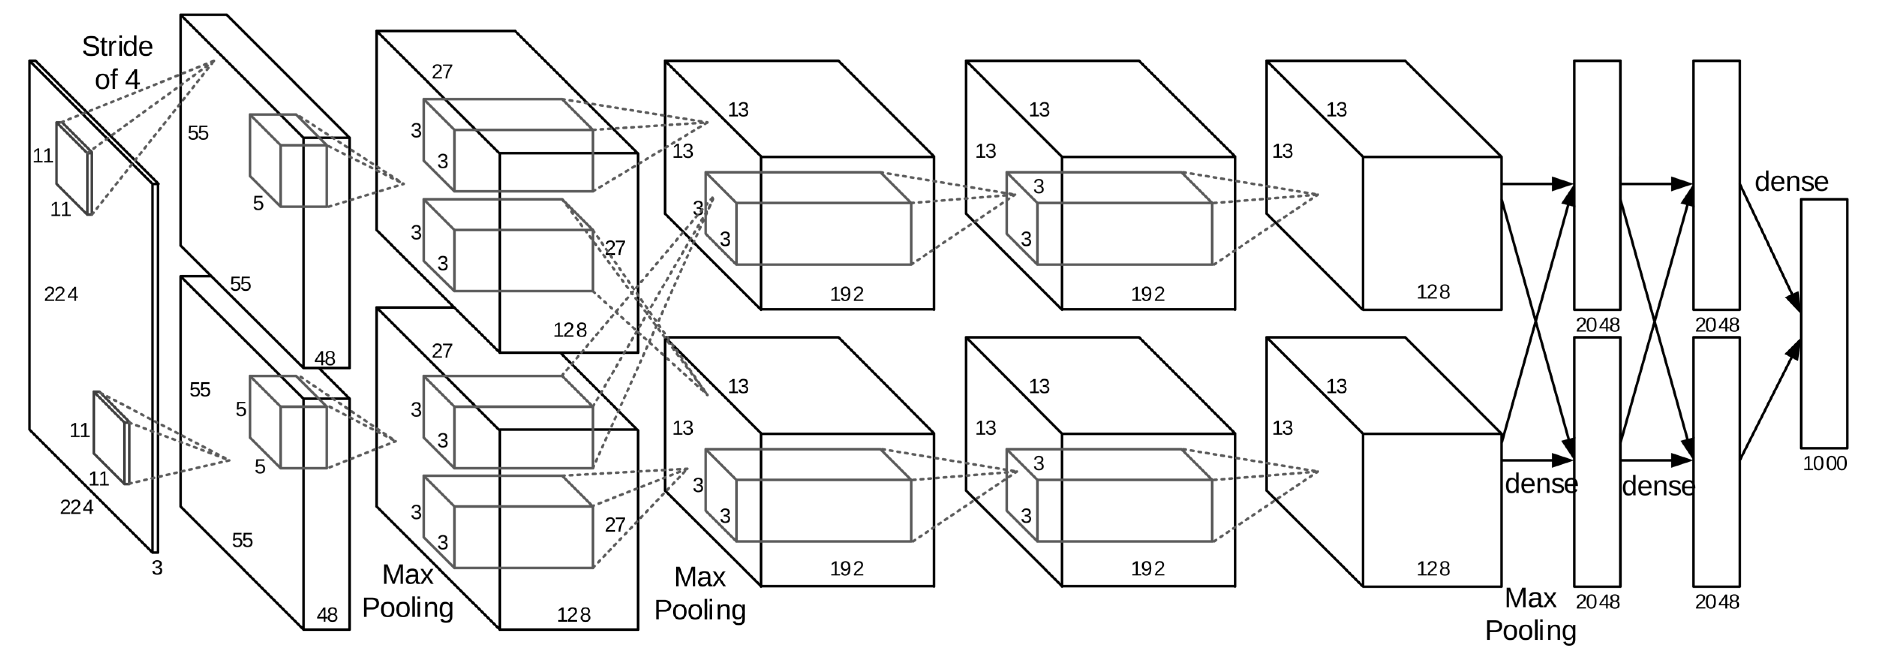
\includegraphics[width=1.0\textwidth]{figures/alexnet.pdf}
    \caption{AlexNet模型结构示意图 \cite{krizhevsky2012imagenet}}\label{figure:figure17}
\end{figure}

AlexNet模型在2012年ImageNet大赛上一举夺冠并由此开启了深度学习的新时代,它也为后续的CNN模型研究奠定了基础,其模型结构如图\ref{figure:figure17}所示。AlexNet模型主要由5个卷积层、3个池化层和3个全连接层组成。其中,AlexNet的卷积层和全连接层包含了模型所有权重,它们的参数信息见表\ref{table:table7}。

\begin{table}[htbp]
  \centering
  \caption{AlexNet模型结构中的卷积层和全连接层}
  \label{table:table7}
\resizebox{1.0\textwidth}{!}{
  \begin{tabular}{ccc}
    \toprule
      名称 & 类型 & 描述\\
    \midrule
      conv1 & 卷积层 & 输入:$3\times227\times227$,卷积核:$96\times3\times11\times11$,步长:4,padding:0,输出:$96\times55\times55$ \\
      conv2 & 卷积层 & 输入:$96\times27\times27$,卷积核:$256\times96\times5\times5$,步长:1,padding:2,输出:$256\times27\times27$\\
      conv3 & 卷积层 & 输入:$256\times13\times13$,卷积核:$384\times256\times3\times3$,步长:1,padding:1,输出:$384\times13\times13$ \\
      conv4 & 卷积层 & 输入:$384\times13\times13$,卷积核:$384\times384\times3\times3$,步长:1,padding:1,输出:$384\times13\times13$\\
      conv5 & 卷积层 & 输入:$384\times13\times13$,卷积核:$256\times384\times3\times3$,步长:1,padding:1,输出:$256\times13\times13$\\
      fc6 & 全连接层 & 输入:9216, 输出:4096 \\
      fc7 & 全连接层 & 输入:4096, 输出:4096 \\
      fc8 & 全连接层 & 输入:4096, 输出:1000 \\
    \bottomrule
  \end{tabular}
}
\end{table}

图\ref{figure:figure18}显示了AlexNet模型分别在ODROID-XU3平台CPU和GPU上进行单张图片推断的运行时间、能耗和平均功耗对比。与图\ref{figure:figure16}中LeNet-5模型的推断运行相比,AlexNet模型在手机GPU上执行前向推断相较于手机CPU而言性能加速比可达15。从功耗角度分析可得,AlexNet模型在手机GPU上执行前向推断时手机GPU的平均功耗(1.31瓦)可接近其峰值。这也说明了手机GPU在执行AlexNet这种结构较为复杂的CNN模型推断时加速效果更加明显。虽然AlexNet模型在手机GPU上执行前向推断的平均功耗比LeNet-5模型增加了1瓦,但是其仍然只是使用CPU执行推断时功耗的一半,也因此其能耗只达到了使用CPU推断的1/30。由表\ref{table:table8}显示的EDP值可知,相较于手机CPU而言,使用手机GPU执行AlexNet模型推断时能效可提升472倍以上。这充分显示了手机GPU在执行卷积神经网络计算上的优势。

\begin{figure}[htbp]
\begin{minipage}[b]{.6\linewidth}
    \begin{center}
    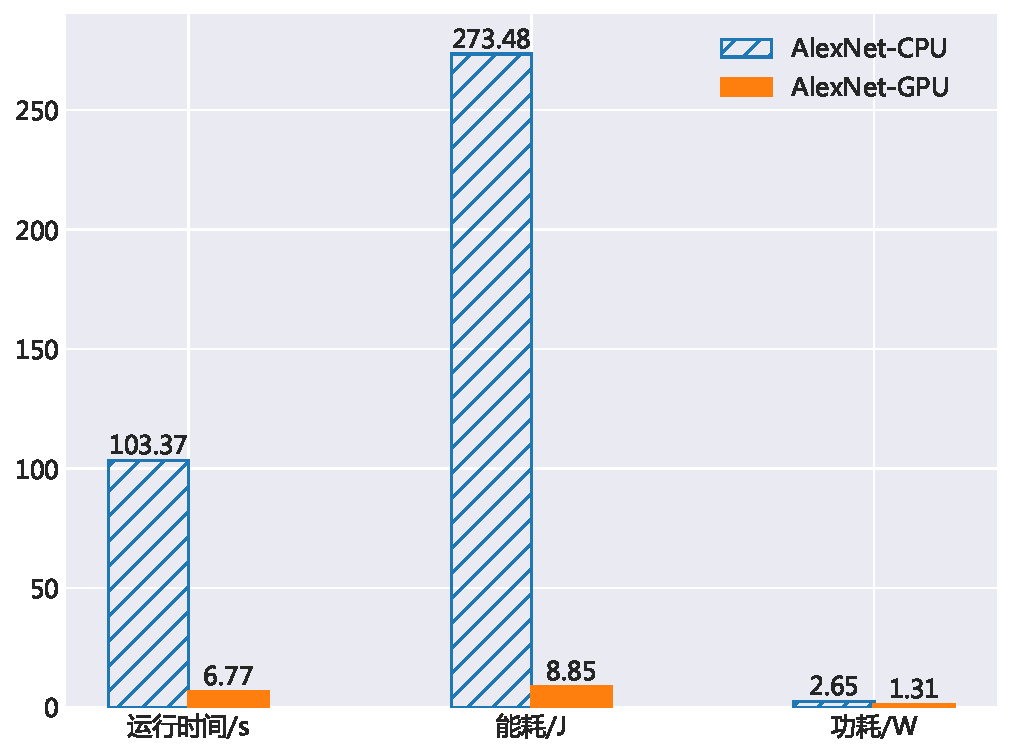
\includegraphics[height=0.65\textwidth]{figures/alexnet_energy.pdf}
    \end{center}
    \captionsetup{font={small}}
    \caption{AlexNet单张图片推断运行时间、能耗和 \\ 平均功耗对比}\label{figure:figure18}
\end{minipage}
\begin{minipage}[b]{.4\linewidth}
\centering
\resizebox{1.0\textwidth}{!}{
\begin{tabular}{cc}
    \toprule
      运行处理器 & EDP(Joules*seconds) \\
    \midrule
      CPU & 28268.24 \\
      GPU & 59.84 \\
    \bottomrule
\end{tabular}
}
\captionsetup{font={small}}
\captionof{table}{AlexNet分别于手机GPU和CPU上运行时能效对比}\label{table:table8}
\end{minipage}
\end{figure}

%\begin{figure}[htbp]
%    \centering
%    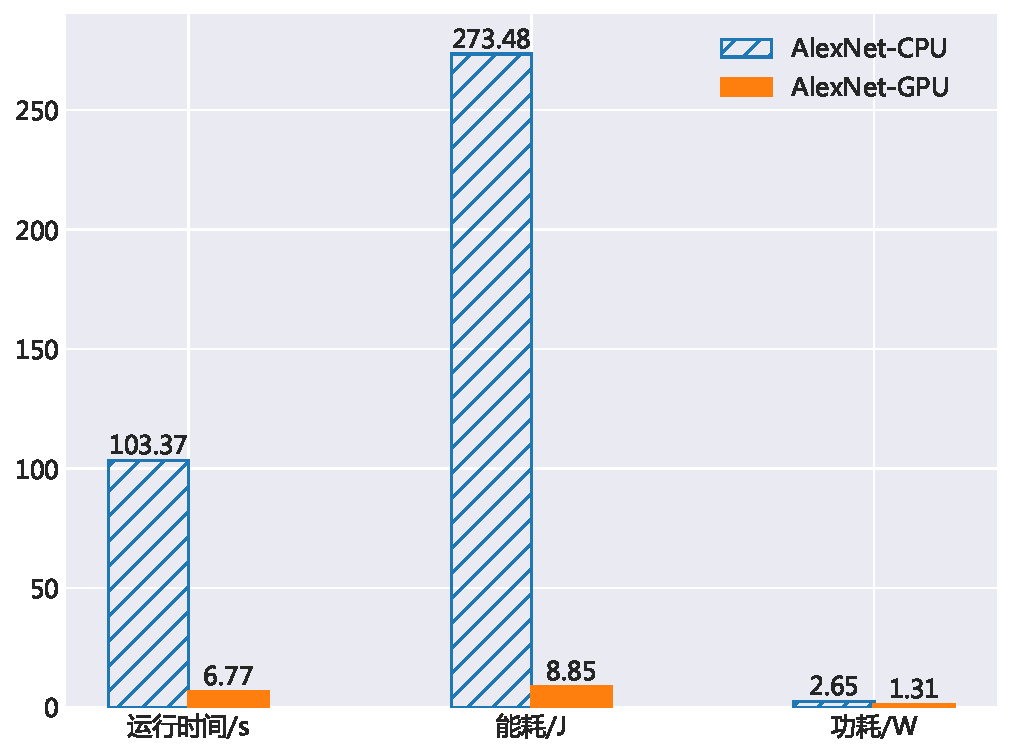
\includegraphics[height=0.45\textwidth]{figures/alexnet_energy.pdf}
%    \caption{ODROID-XU3平台上AlexNet单张图片推断运行时间、能耗和平均功耗对比}\label{figure:figure18}
%\end{figure}
%
%\begin{table}[htbp]
%  \centering
%  \caption{AlexNet分别于手机GPU和CPU上运行时能效对比}
%  \label{table:table8}
%  \begin{tabular}{cc}
%    \toprule
%      运行处理器 & EDP(Joules*seconds) \\
%    \midrule
%      CPU & 28268.24 \\
%      GPU & 59.84 \\
%    \bottomrule
%  \end{tabular}
%\end{table}

为了验证本文所开发CNN推断时库的可移植性与兼容性,本文在Open-Q™ 820开发套件上也重构了AlexNet模型。图\ref{figure:figure19}显示了AlexNet模型分别于ODROID-XU3平台和Open-Q™ 820开发套件上进行单张图片推断的CPU运行时间和GPU运行时间。对比在两个平台上使用手机CPU执行AlexNet前向推断的运行时间可知,骁龙820的CPU相较于三星\texttt{Exynos5422}的CPU在计算性能上提升了4倍有余。而当使用手机GPU执行CNN前向推断时,骁龙820的处理速度更是提升了11倍多,这使得在手机端完成一次完整的AlexNet前向推断仅需要580毫秒。由此可以看出,手机SoC中的CPU和GPU处理性能都在日趋强大,这为深度学习模型(如卷积神经网络)在手机本地完成离线推断奠定了基础。

\begin{figure}[htbp]
    \centering
    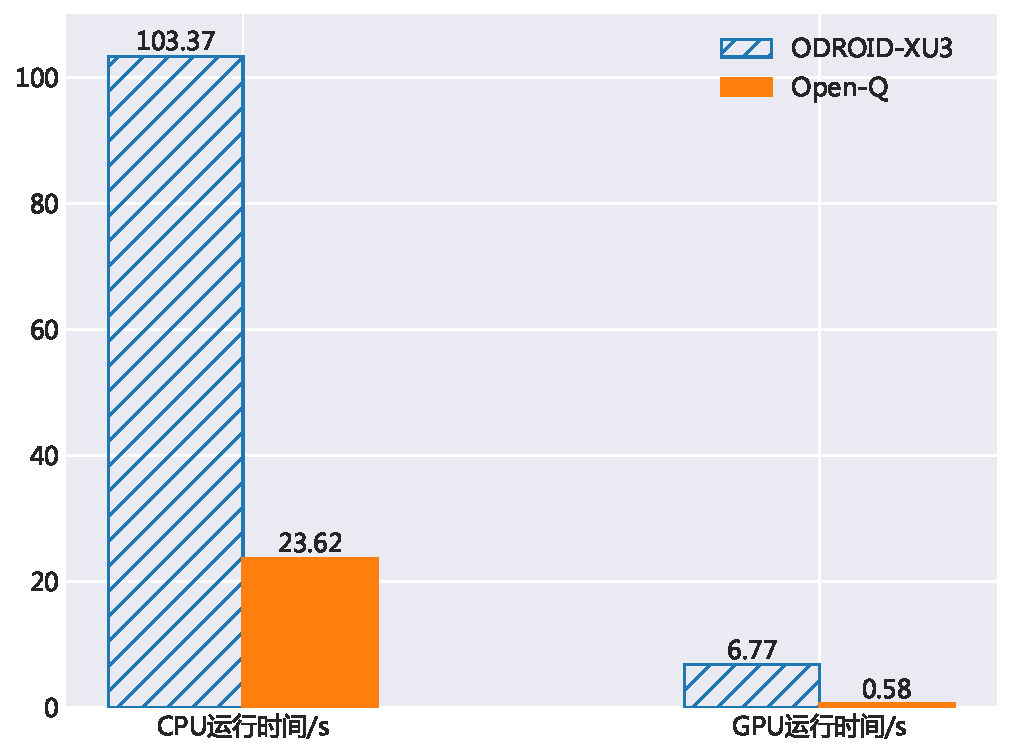
\includegraphics[height=0.4\textwidth]{figures/open_q.pdf}
    \caption{不同平台上AlexNet单张图片推断运行时间对比}\label{figure:figure19}
\end{figure}


\section{基于“剪枝-重训”的层压缩优化}

神经网络是一种典型的过参数化模型,其通常包含着大量的冗余参数,例如:AlexNet模型采用Caffe框架的caffemodel格式进行存储时大小约为244MB。这种过多的冗余参数会导致计算和内存占用两方面的浪费。另一方面,手机相较于桌面电脑而言,其往往配备着较低容量的内存,如华为Mate 9 Pro和三星 Galaxy S8的内存大小均为4GB。分析卷积神经网络模型权重参数分布可知,全连接层参数占了整个网络参数的绝大部分,如AlexNet模型中全连接层参数占整个网络参数的95\%以上。因此,为了降低CNN模型在手机端进行前向推断时的内存占用开销,本文采用“剪枝-重训”方法对CNN模型的全连接层参数进行压缩。

“剪枝”的主体思想就是将不重要的冗余权重连接删除,只保留网络模型中最重要的连接部分。本文参考《Learning both weights and connections for efficient neural network》\cite{han2015learning}文章中的通用剪枝思想将权值绝对值大小低于某一阈值的连接视为不重要的冗余连接。“重训”即剪枝后重新训练,这主要为了保证剪枝操作不会造成网络模型的精度损失。很明显,如果直接删除网络模型中的部分连接而不做重新训练处理,那么模型的精度就会下降。故而,为了保证网络模型的精度不变,需要对剪枝后的网络进行重新训练。

在对网络模型进行剪枝时,必须要确定待剪枝层的权重连接保留率,即保留待剪枝层的权重连接数量。一般来说,权重连接数越多的层则其需要剪枝掉的连接数也应该越多,即权重连接保留率越低。试错实验法是目前用来确定权重连接保留率的常用方法,即对每一个待剪枝层L进行如下操作:
\begin{enumerate}
  \item 除L层以外,将其他层的权重连接保留率都设置为1,即除L层外不剪枝;
  \item 以从高到低的方式设置L层权重连接保留率大小(如从0.95以步长0.05递减到0.05);
  \item 使用第二步设置的每一个权重连接保留率对L层进行剪枝,并对剪枝后的网络模型于测试集上进行推断以获取剪枝后模型的精度;
  \item 根据模型精度的变化确定L层的最低权重连接保留率。
\end{enumerate}


\subsection{模型剪枝流程}

\begin{figure}[htbp]
    \centering
    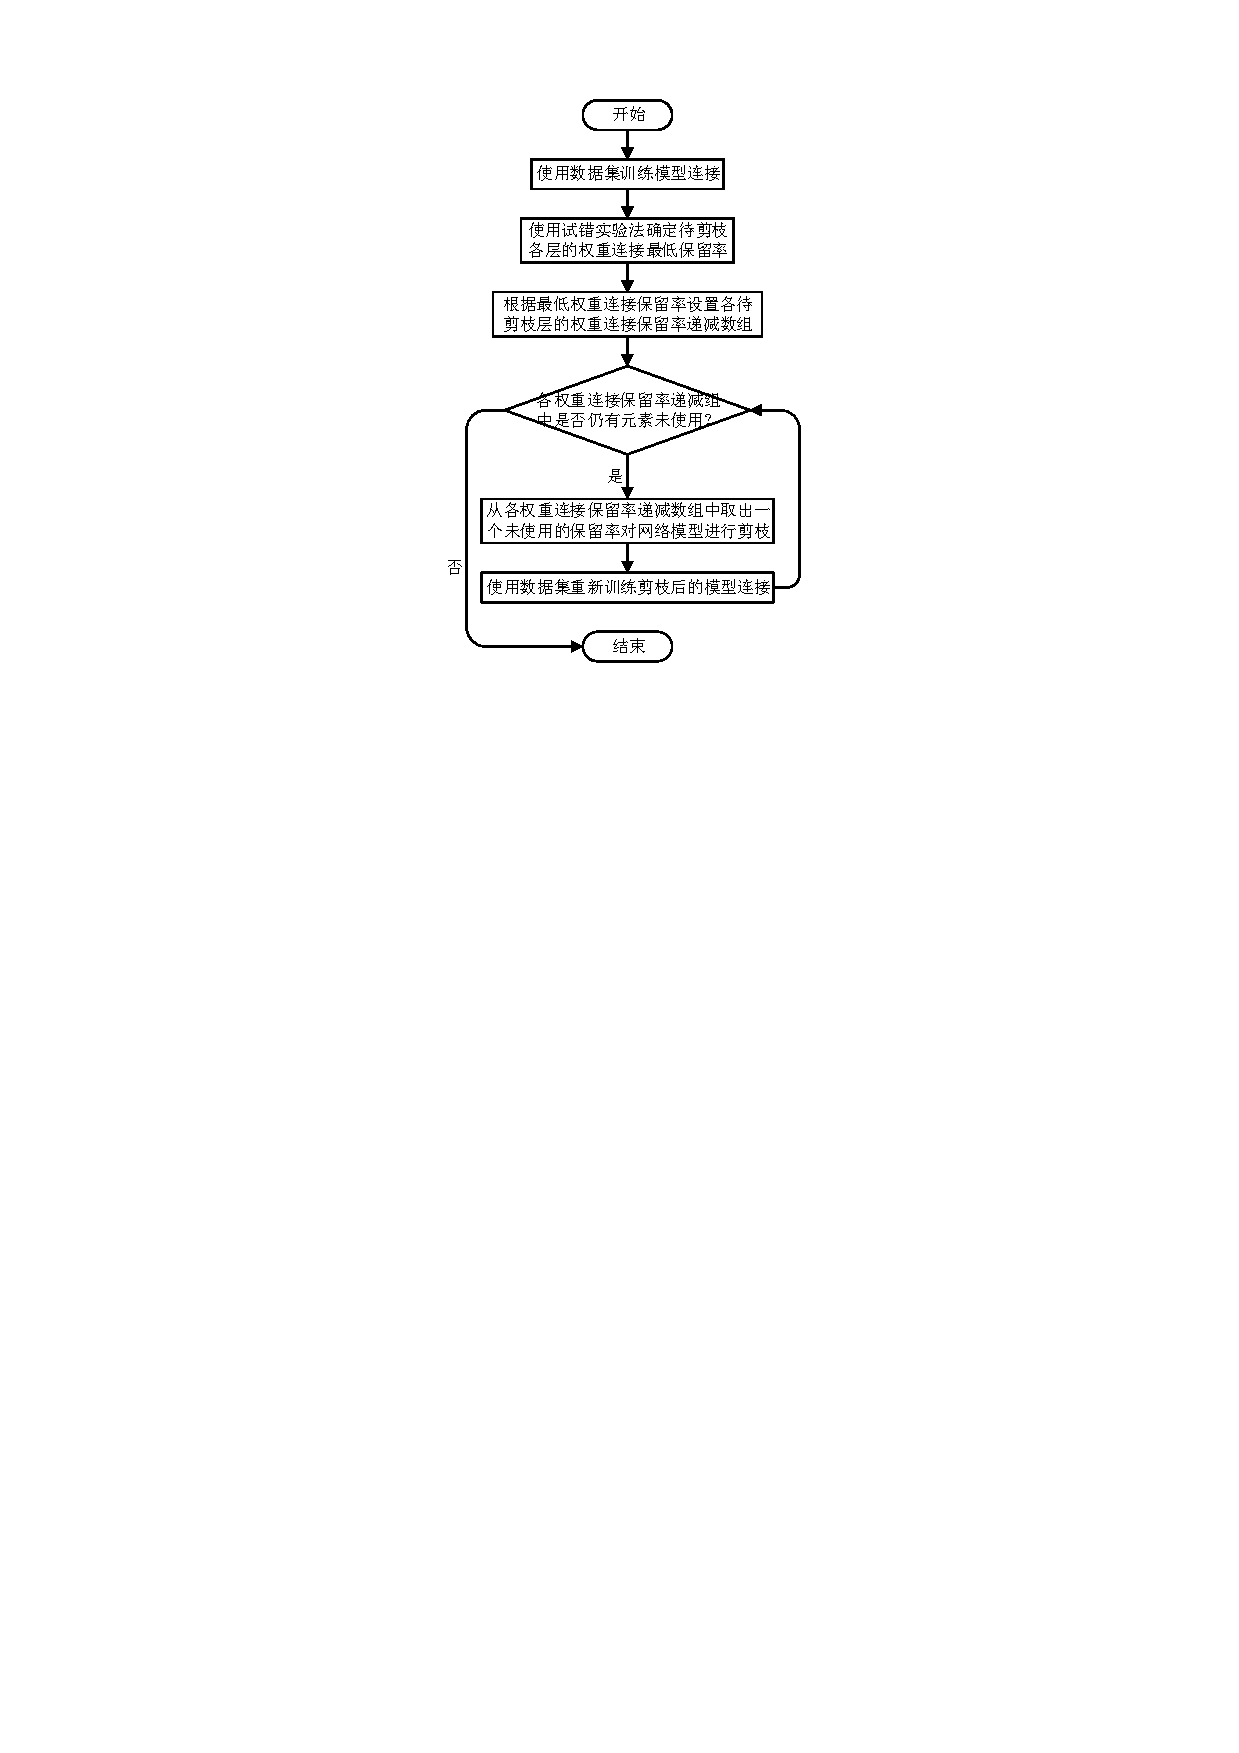
\includegraphics[height=0.8\textwidth]{figures/prune.pdf}
    \caption{“剪枝-重训”流程概览}\label{figure:figure20}
\end{figure}

图\ref{figure:figure20}描述了模型“剪枝-重训”的整体流程。首先,使用数据的训练集对CNN模型进行训练以获得稠密权重连接。接着,使用试错实验法确定各待剪枝层的最低权重连接保留率。本文采用逐渐降低权重连接保留率的方式对网络模型进行迭代“剪枝-重训”,而不是使用最低权重连接保留率一次性对模型进行剪枝。因此,本文根据试错实验法得到的最低权重连接保留率来设置各待剪枝层的权重连接保留率递减数组。举例来说,对于某一层L,使用试错实验法发现将其保留率设为0.1对模型整体精度损失不大,则L层的权重连接保留率递减数组可设置成$[0.95,0.9,0.85,...,0.15,0.1]$。最后,对各待剪枝层的权重连接保留率递减数组进行迭代:每次取出一组保留率对模型进行“剪枝-重训”操作,直至各待剪枝层的权重连接达到目标保留数量。

根据图\ref{figure:figure20}所描述的流程,本文对Caffe框架源码进行了修改,使其支持上述的“剪枝-重训”操作,并针对LeNet-5模型和AlexNet模型进行了实验。另外,对于稀疏矩阵,本文采用CSR格式进行存储,即只保存稀疏矩阵的非零值、行的范围以及非零值的列下标。

\subsection{LeNet-5模型剪枝}

图\ref{figure:figure21}显示了LeNet-5模型精度随两个全连接层权重连接保留率的变化趋势。从趋势图上可以看出:全连接层ip1包含的冗余连接数过多,所以减少其权重连接对整个模型的前向推断精度影响不大;而全连接层ip2受剪枝影响较大,当只保留其5\%的权重连接时会导致整个模型的推断精度下降到82\%左右。因此,为了保证剪枝后LeNet-5模型的推断精度仍在90\%以上,本文将全连接层ip1和ip2的最低权重连接保留率分别设为0.05和0.1。

\begin{figure}[htbp]
    \centering
    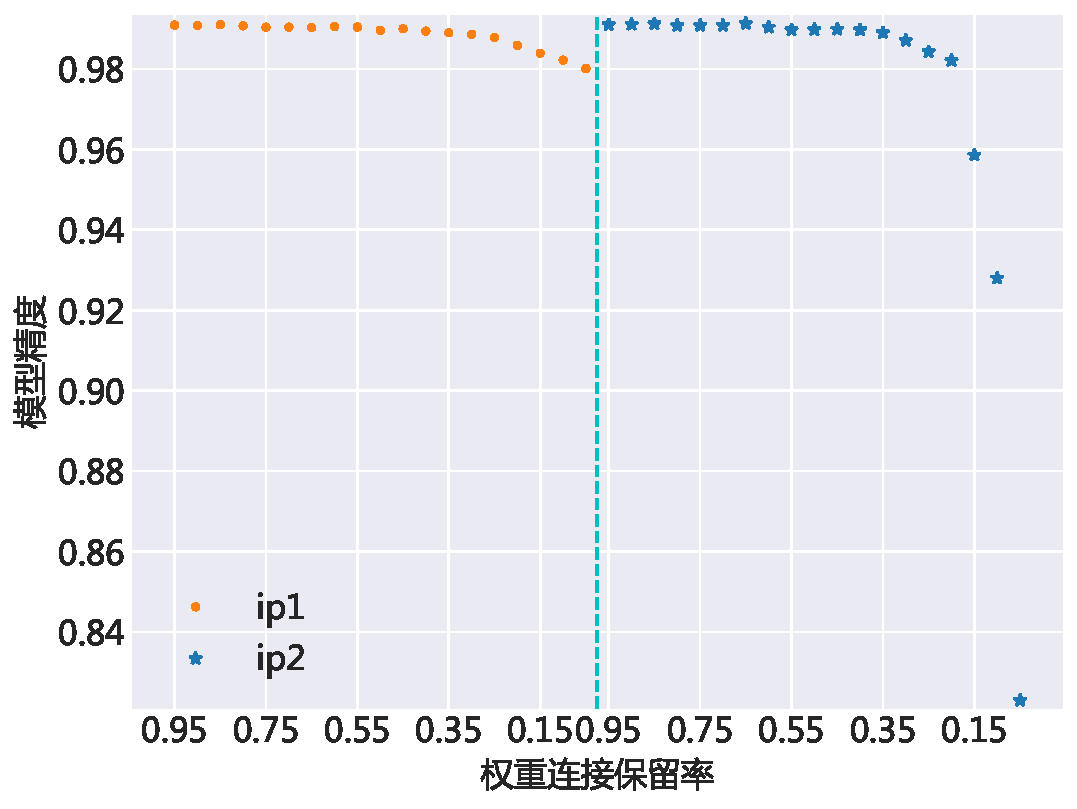
\includegraphics[height=0.4\textwidth]{figures/lenet_pruned_threshold.pdf}
    \caption{LeNet-5模型精度随全连接层权重连接保留率的变化曲线}\label{figure:figure21}
\end{figure}

使用图\ref{figure:figure20}所示的“剪枝-重训”流程对LeNet-5模型进行剪枝后,可以发现其模型推断精度仍可高达99.05\%,这几乎没有导致精度上任何损失。剪枝后的模型经CSR格式进行存储后,模型大小仅为原始模型的15.65\%。在此需要说明,虽然全连接层ip1和ip2的权重参数分别减少了95\%和90\%,但是由于CSR存储格式需要存储稀疏矩阵中所有非零值元素的两类信息(元素值和其对应的列下标),所以模型大小仅压缩到原始模型的15\%左右。由LeNet-5模型所有全连接层剪枝前后的权重分布对比图\ref{figure:figure22}可知,LeNet-5模型经剪枝后全连接层的权重只有很少一部分值为非零值,这说明剪枝操作确实将原有的稠密权重矩阵转换为了稀疏权重矩阵。

\begin{figure}[htbp]
    \centering
    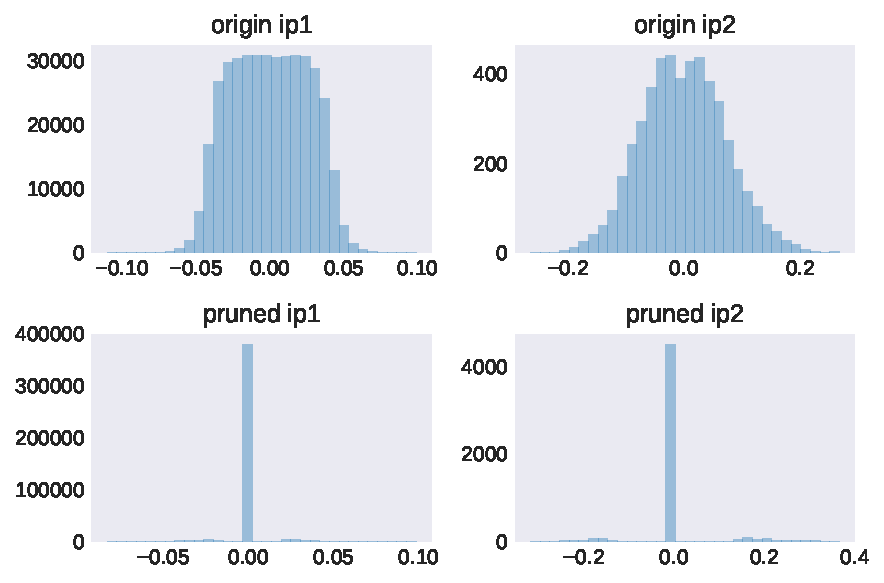
\includegraphics[height=0.41\textwidth]{figures/lenet_pruned_weights.pdf}
    \caption{LeNet-5模型全连接层剪枝前后权重分布对比}\label{figure:figure22}
\end{figure}

%LeNet-5模型结构比较简单,因此其原始大小也仅1.7MB,对其进行压缩意义并非很大。因此,接下来本文使用“剪枝-重训”方法对AlexNet模型进行压缩。

\subsection{AlexNet模型剪枝}

与LeNet模型剪枝类似,本文首先使用试错实验法确定AlexNet模型各全连接层的最低权重连接保留率,其模型精度随不同层权重连接保留率的变化趋势如图\ref{figure:figure23}所示。通过对比分析可知,fc6层的剪枝对模型精度影响最大,而fc8层的剪枝对模型精度影响较小。为了保证剪枝后模型的top-1准确率仍在50\%以上,本文将全连接层fc6、fc7和fc8的最低权重连接保留率均设置成0.15。需要说明的是,本文所使用的AlexNet模型剪枝前在ImageNet\cite{imagenet.org}数据集上的top-1准确率为55.78\%。

\begin{figure}[htbp]
    \centering
    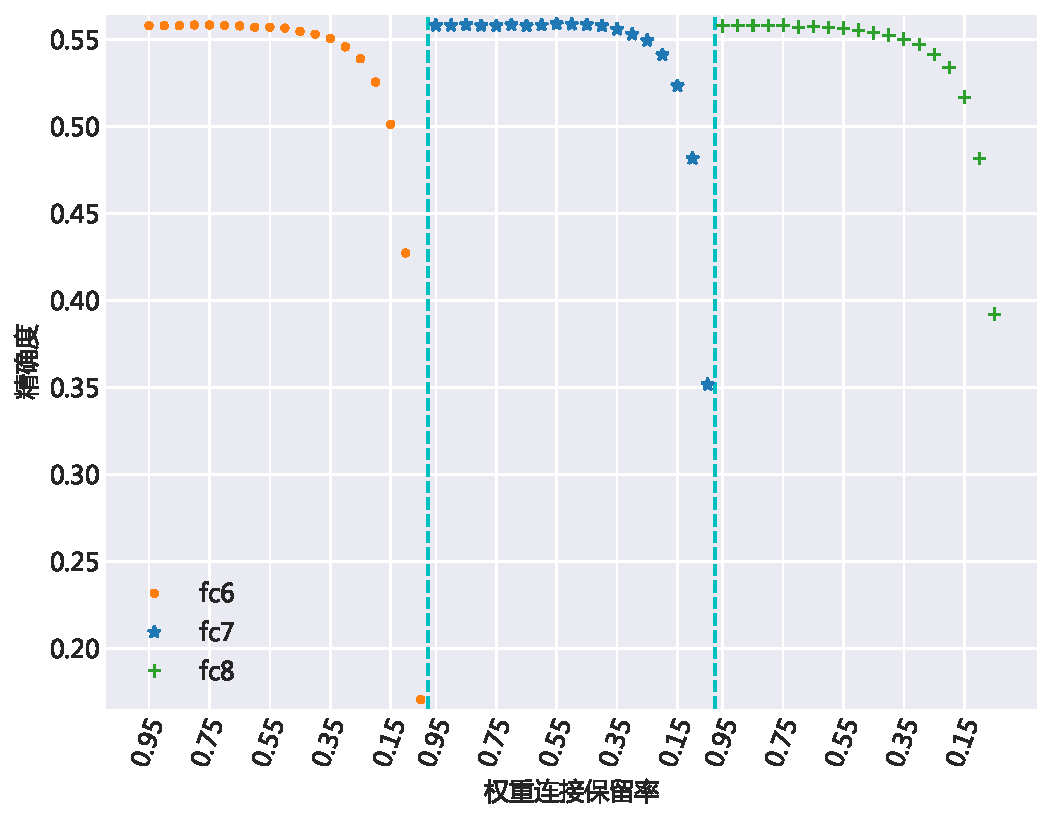
\includegraphics[height=0.4\textwidth]{figures/alexnet_pruned_threshold.pdf}
    \caption{AlexNet模型精度随全连接层权重连接保留率的变化曲线}\label{figure:figure23}
\end{figure}

经多次“剪枝-重训”操作后,AlexNet模型的所有全连接层都仅保留了原有权重的15\%,而模型的top-1准确率变成了54.80\%,模型精度仅下降了0.98\%。因为实验中每次剪枝后的对模型仅仅重新训练了10000次,所以这可能造成了模型精度0.98\%的损失。如果增加每次剪枝后模型的重新训练次数,模型的精度损失就会减少。使用CSR格式对剪枝后的AlexNet模型进行存储,其模型大小约为85MB,这比原始模型大小减少了约159MB,仅占原始模型大小的34.8\%。图\ref{figure:figure24}显示了AlexNet模型的各全连接层剪枝前后权重分布对比。从分布图中可以明显看出,经剪枝后,AlexNet模型的所有全连接层的权重值仅有很少一部分值不为0。

\begin{figure}[htbp]
    \centering
    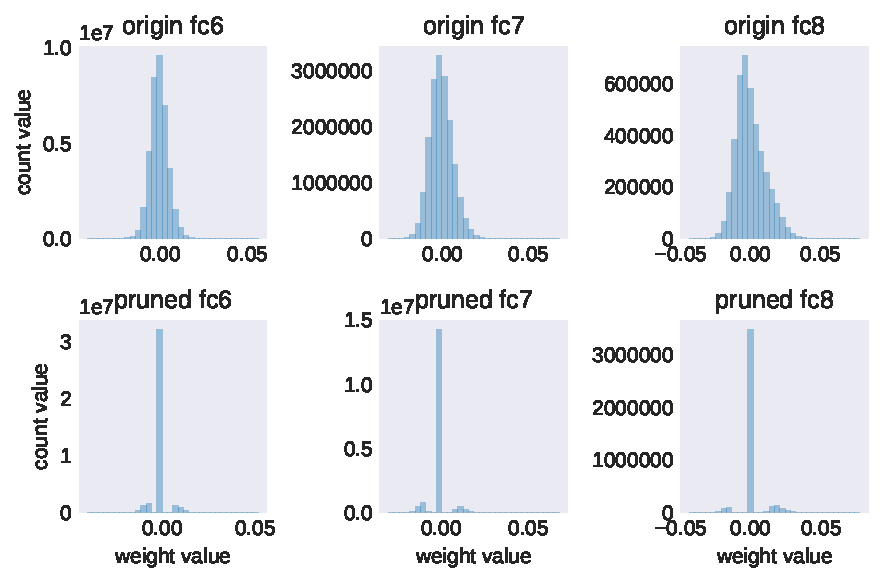
\includegraphics[height=0.41\textwidth]{figures/alexnet_pruned_weights.pdf}
    \caption{AlexNet模型全连接层剪枝前后权重分布对比}\label{figure:figure24}
\end{figure}


基于ODROID-XU3平台,本文分析比较了AlexNet模型在剪枝前后的首次加载时间、能耗和平均功耗变化,结果如图\ref{figure:figure27}所示。分析图\ref{figure:figure27}中的数据可知,对AlexNet模型的全连接层进行剪枝后(仅保留全连接层原有权重的15\%),模型的首次加载时间减少了60\%,并且内存读取操作所产生的能耗也降为原来的一半。这说明,对神经网络模型进行剪枝操作不仅可以降低模型的内存占用还可以加快模型的加载速度并同时减少内存能耗开销。

\begin{figure}[htbp]
    \centering
    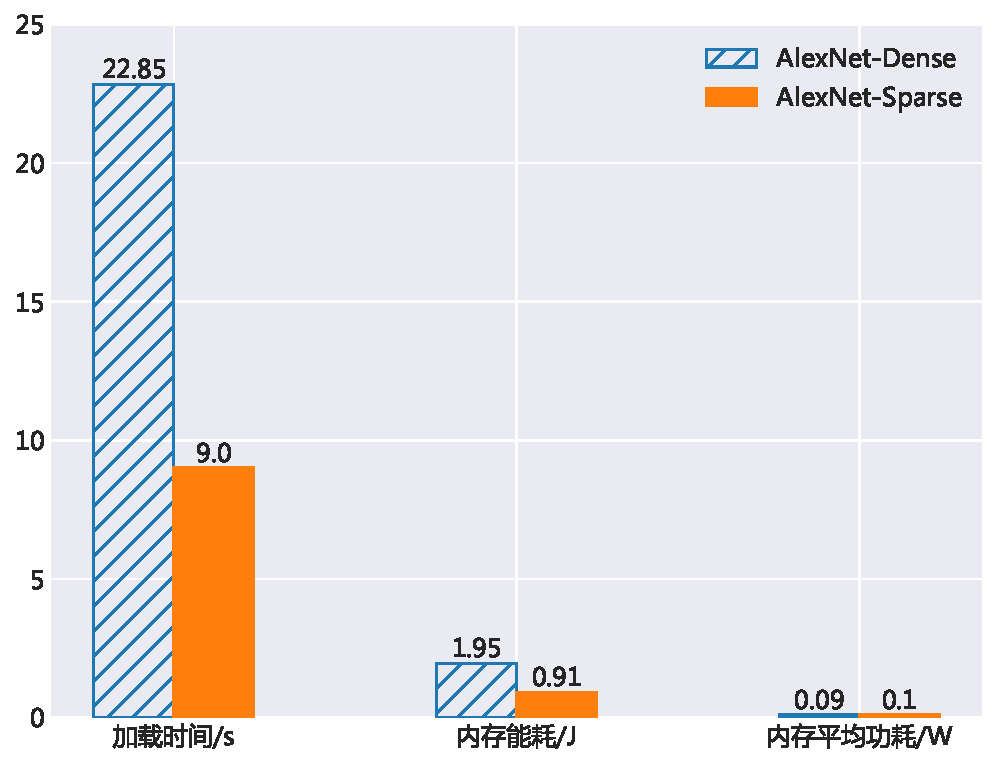
\includegraphics[height=0.4\textwidth]{figures/alexnet_init.pdf}
    \caption{剪枝前后AlexNet首次加载时间、能耗和平均功耗对比}\label{figure:figure27}
\end{figure}

\subsection{手机端SpMV的实现}

对于剪枝压缩后的卷积神经网络模型,本文使用稀疏矩阵向量乘(SpMV)代替原全连接层的稠密矩阵向量乘(内积操作)。对于一个使用CSR格式存储的稀疏矩阵与一个向量的乘积操作,其实现伪代码如算法\ref{algo:algorithm7}所示。

\begin{algorithm}[htbp]
  \small
  \SetAlgoLined
  \KwData{num\_rows, ptr, indices, data, bias, vec, out}
    \begin{spacing}{0.9}
    num\_rows表示稀疏矩阵的总行数\;
    ptr, indices, data分别表示行的范围、非零值的列下标以及稀疏矩阵的非零值\;
    bias, vec, out分别表示偏置矩阵、乘数向量以及乘积结果\;
  \For{row in 0 ... num\_rows-1}{
        tmp = 0\;
        计算第row行的非零值下标范围[start\_row, end\_row)\;
        \For{j in start\_row ... end\_row-1}{
            temp += data[j] * vec[indices[j]];
        }
        out[row] = temp + bias[row];
  }
    \end{spacing}
  \caption{SpMV的实现伪代码}
  \label{algo:algorithm7}
\end{algorithm}

根据算法\ref{algo:algorithm7}所述过程,本文分别于手机GPU和CPU上实现了稀疏矩阵向量乘操作。图\ref{figure:figure25}显示了于ODROID-XU3平台的GPU和CPU上进行稀疏矩阵向量乘和使用内积进行稠密矩阵向量乘的运行时间、能耗和平均功耗对比。实验中,矩阵维度为$4096 \times 9216$,向量维度为$9216 \times 1$,矩阵的非零值比重为15\%。

\begin{figure}[htbp]
    \centering
    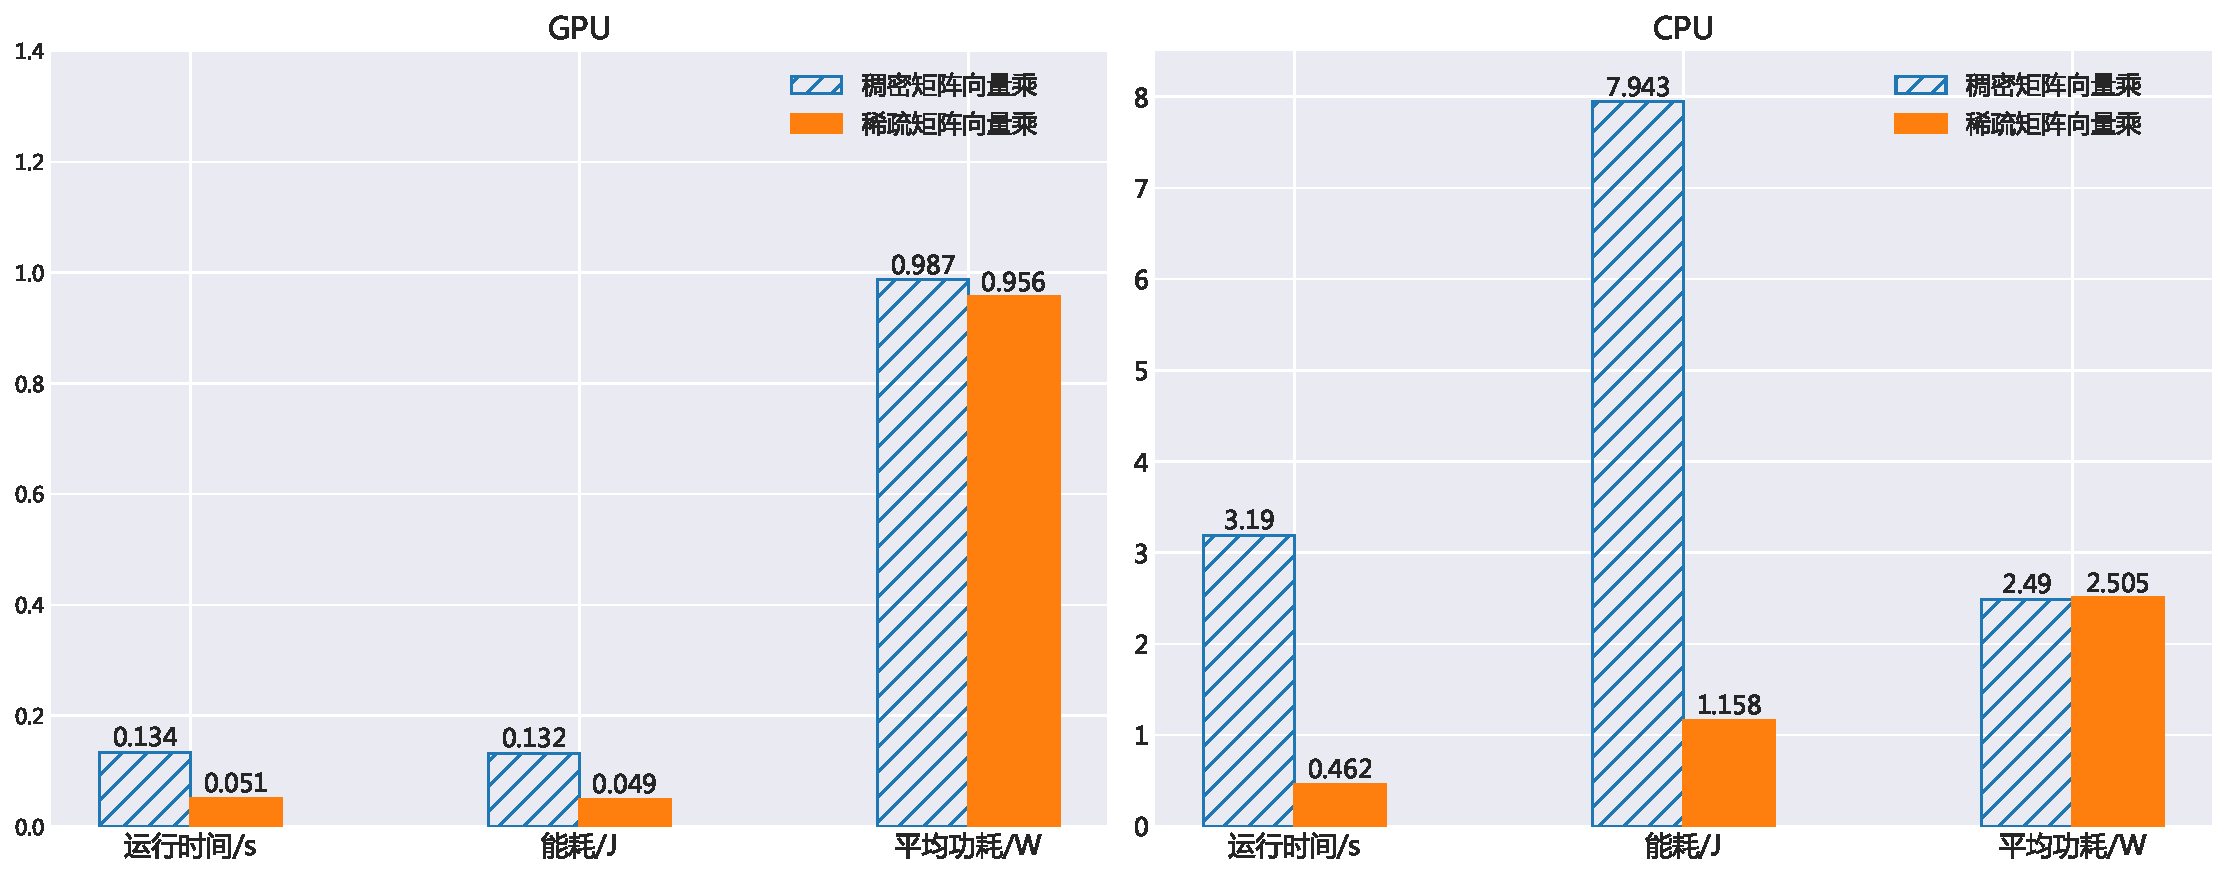
\includegraphics[width=1.0\textwidth]{figures/spmv.pdf}
    \caption{稠密矩阵和稀疏矩阵向量乘的运行时间、能耗和平均功耗对比}\label{figure:figure25}
\end{figure}

由图\ref{figure:figure25}可知,GPU上使用SpMV代替内积运算,可将矩阵向量乘操作的运行速度提升2.63倍,并且完成乘积操作也只需原能耗的1/3左右。而在CPU上使用SpMV操作更可将运行时间和能耗均降为原来的1/7左右。这充分说明矩阵的压缩操作不仅可以带来内存占用和能耗的降低,更可以提升矩阵乘积的计算速度。


\begin{figure}[htbp]
    \centering
    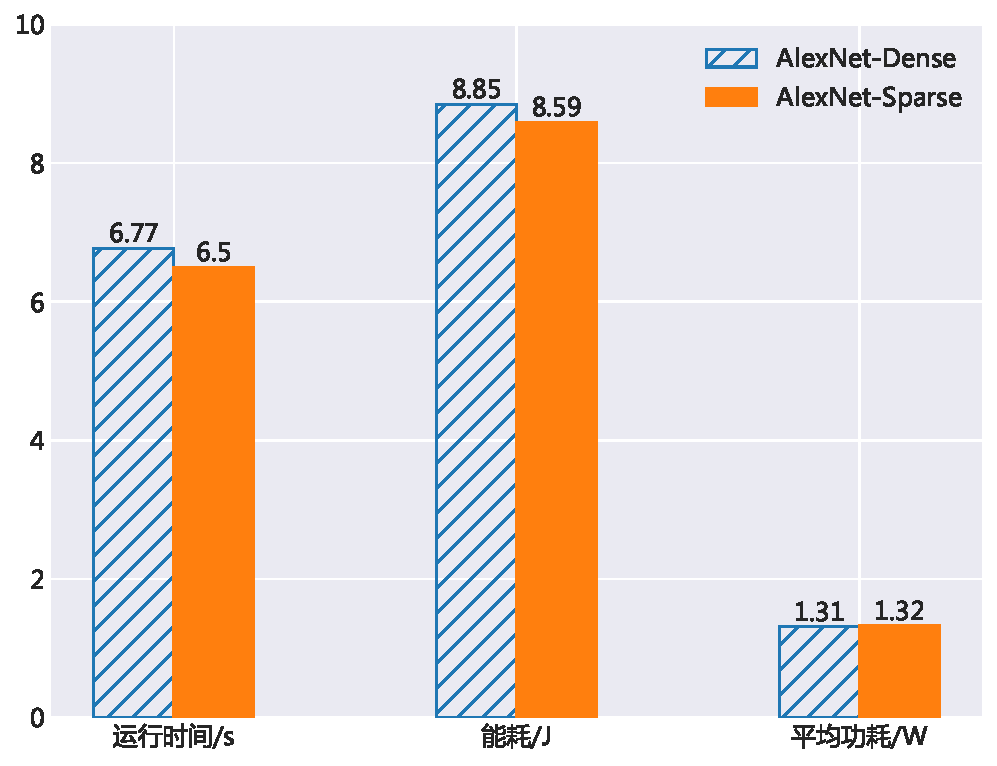
\includegraphics[height=0.4\textwidth]{figures/alexnet_sparse.pdf}
    \caption{AlexNet剪枝前后单张图片推断运行时间、能耗和平均功耗对比}\label{figure:figure26}
\end{figure}

对AlexNet模型全连接层进行剪枝并使用SpMV代替全连接层的内积算子后,再次于ODROID-XU3平台上测量其推断单张图片的运行时间、能耗和平均功耗,结果如图\ref{figure:figure26}中的AlexNet-Sparse数据系列所示。与剪枝前的稠密AlexNet模型相比,稀疏AlexNet模型的前向推断时间、能耗都有所降低,但降低幅度不大。这主要是因为全连接层的计算时间占整个CNN推断执行时间的比重较小。

\subsection{与CNNdroid的对比}

CNNdroid是Seyyed等人开发的基于GPU加速的CNN推断时库。根据CNNdroid作者提供的源码,本文在Open-Q™ 820平台上使用其运行了AlexNet模型的前向推断过程,并将运行结果与本文所开发的CNN推断时库(使用GPU)做对比,结果如图\ref{figure:figuredroid}所示。实验之所以未选择使用ODROID-XU3平台,是因为CNNdroid在ODROID-XU3平台上不能成功执行AlexNet模型推断,这可能与CNNdroid运行时内存占用过大或其使用的GPU编程框架存在限制条件有关。

\begin{figure}[htbp]
    \centering
    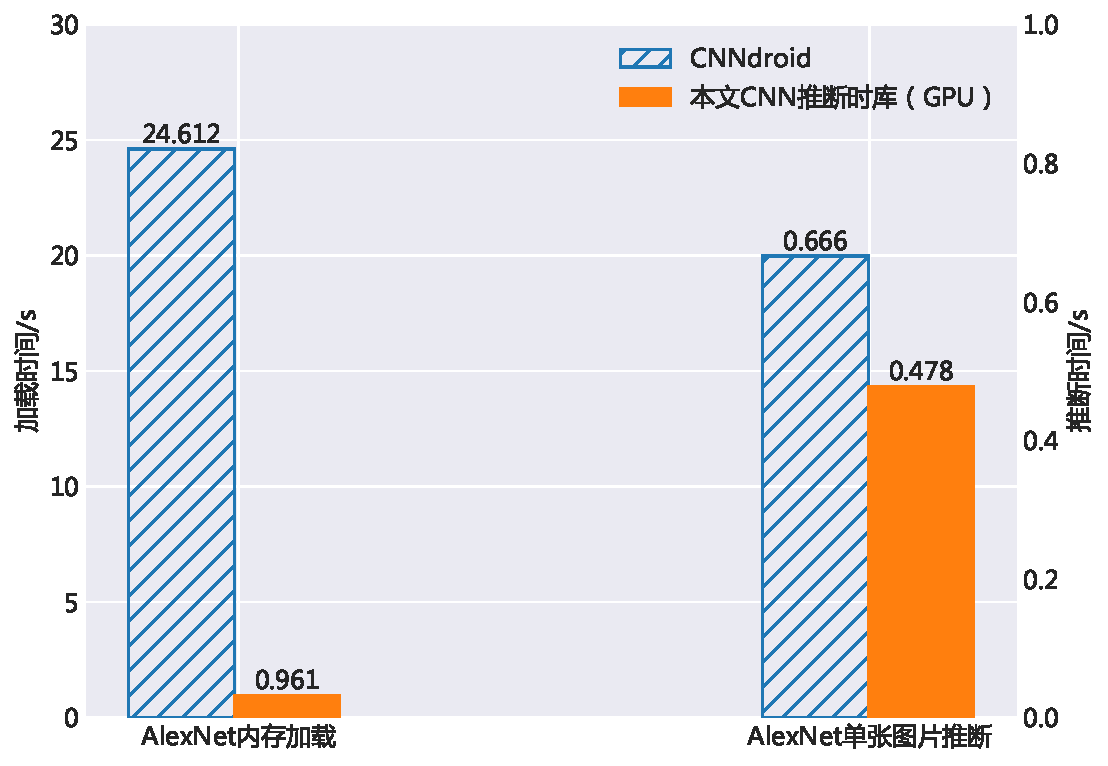
\includegraphics[height=0.41\textwidth]{figures/cnndroid.pdf}
    \caption{本文CNN推断时库与CNNdroid的对比}\label{figure:figuredroid}
\end{figure}

从图\ref{figure:figuredroid}中的AlexNet模型在两个推断时库中的内存加载时间可以看出,CNNdroid的AlexNet模型内存加载时间远高于本文所开发的CNN推断时库(大约是本文CNN推断时库的25.6倍)。根据表\ref{table:tabledroid}中所示AlexNet模型在两个推断时库中的SD卡存储占用和内存占用可知,CNNdroid不仅没有对AlexNet模型进行压缩,而且其采用的模型存储格式比Caffe框架的caffemodel格式所需存储占用更大。这不仅导致了AlexNet模型对SD卡存储占用和内存占用的需求极高,而且造成了图\ref{figure:figuredroid}中模型加载时间过长的原因。由此可见,本文所采用的“剪枝-重训”模型压缩操作的必要性。


\begin{table}[htbp]
  \centering
  \caption{AlexNet模型的存储占用和内存占用需求}
  \label{table:tabledroid}
  \begin{tabular}{ccc}
    \toprule
       & SD卡存储占用(MB)& 内存占用(MB) \\
    \midrule
      CNNdroid & $290$ & $\sim 300$ \\
      本文CNN推断时库& $85$ & $\sim 90$ \\
    \bottomrule
  \end{tabular}
\end{table}


图\ref{figure:figuredroid}也显示了CNNdroid和本文CNN推断时库的AlexNet模型单张图片推断时间,它们分别是两个推断时库执行100次AlexNet模型推断的平均运行时间。对比两个推断时库的模型推断执行时间可知,本文所开发的CNN推断时库因为使用了模型压缩和SpMV等优化操作,运行AlexNet模型推断的速度要快于CNNdroid(加速比约为1.4)。

通过以上分析可以发现,本文所采用的模型压缩和SpMV等优化操作使得所开发的CNN推断时库无论是在内存加载速度还是在模型推断性能上均高于CNNdroid。虽然对CNN模型权重进行“剪枝-重训”压缩可能会造成一定的模型推断精度损失,但是这种精度损失很小(本文压缩后AlexNet模型精度下降不足1\%),而且使用合理地剪枝以及充分地再训练操作也可以避免这种模型的精度损失。




\section{本章小结}

本章主要介绍了基于手机GPU加速和模型压缩的CNN前向推断能效优化方法。3.1节对CNN模型前向推断过程中所使用的基本算子进行了分解与手机端的实现,并基于ODROID-XU3平台分析比较了各个基本算子在手机GPU和CPU上的运行时能效。3.2节根据所实现的各种基本算子设计了一套CNN推断时库。基于该推断时库,本文在手机端重构了LeNet-5模型和AlexNet模型,并分析了两个模型在手机GPU和CPU上进行单张图片推断时的能效。3.3节介绍了“剪枝-重训”的模型压缩方法,并实现了对卷积神经网络全连接层权重的压缩。通过对LeNet-5和AlexNet两个模型的剪枝操作,本文验证了使用压缩方法提升CNN模型于手机端运行时能效的有效性。基于压缩后的稀疏网络模型,本文使用稀疏矩阵向量乘操作(SpMV)代替全连接层的内积操作,进一步增强了所开发推断时库在Android平台上的可用性。最后,与CNNdroid的对比实验展示了本文所采用SpMV和模型压缩等优化方法所带来的性能提升。截至本章,本文已经开发了一套可以分别于手机GPU和CPU上运行的CNN推断时库,该库还通过SpMV操作支持经“剪枝-重训”压缩处理的稀疏CNN模型。

\cleardoublepage
